%%%%%%%%%%%%%%%%%%%%%%%%%%%%%%%%%%%%%%%%%
% Journal Article
% LaTeX Template
% Version 1.4 (15/5/16)
%
% This template has been downloaded from:
% http://www.LaTeXTemplates.com
%
% Original author:
% Frits Wenneker (http://www.howtotex.com) with extensive modifications by
% Vel (vel@LaTeXTemplates.com)
%
% License:
% CC BY-NC-SA 3.0 (http://creativecommons.org/licenses/by-nc-sa/3.0/)
%
%%%%%%%%%%%%%%%%%%%%%%%%%%%%%%%%%%%%%%%%%

%----------------------------------------------------------------------------------------
%	PACKAGES AND OTHER DOCUMENT CONFIGURATIONS
%----------------------------------------------------------------------------------------

\documentclass[twoside,a4paper]{article}

\usepackage{blindtext} % Package to generate dummy text throughout this template 

\usepackage[sc]{mathpazo} % Use the Palatino font
\usepackage[T1]{fontenc} % Use 8-bit encoding that has 256 glyphs
\linespread{1.05} % Line spacing - Palatino needs more space between lines
\usepackage{microtype} % Slightly tweak font spacing for aesthetics

\usepackage[english]{babel} % Language hyphenation and typographical rules

\usepackage[hmarginratio=1:1,top=32mm,columnsep=20pt]{geometry} % Document margins
\usepackage[hang, small,labelfont=bf,up,textfont=it,up]{caption} % Custom captions under/above floats in tables or figures
\usepackage{booktabs} % Horizontal rules in tables

\usepackage{lettrine} % The lettrine is the first enlarged letter at the beginning of the text

\usepackage{enumitem} % Customized lists
\setlist[itemize]{noitemsep} % Make itemize lists more compact

\usepackage{abstract} % Allows abstract customization
\renewcommand{\abstractnamefont}{\normalfont\bfseries} % Set the "Abstract" text to bold
\renewcommand{\abstracttextfont}{\normalfont\small\itshape} % Set the abstract itself to small italic text

\usepackage{titlesec} % Allows customization of titles
\renewcommand\thesection{\Roman{section}} % Roman numerals for the sections
\renewcommand\thesubsection{\roman{subsection}} % roman numerals for subsections
\titleformat{\section}[block]{\large\scshape\centering}{\thesection.}{1em}{} % Change the look of the section titles
\titleformat{\subsection}[block]{\large}{\thesubsection.}{1em}{} % Change the look of the section titles

\usepackage{fancyhdr} % Headers and footers
\pagestyle{fancy} % All pages have headers and footers
\fancyhead{} % Blank out the default header
\fancyfoot{} % Blank out the default footer
\fancyhead[C]{Review of Relevant Work for Analyzing default-ability of Home Loan Lenders using Machine Learning Models} % Custom header text
\fancyfoot[RO,LE]{\thepage} % Custom footer text

\usepackage{titling} % Customizing the title section

\usepackage{hyperref} % For hyperlinks in the PDF
\usepackage{graphicx}
\graphicspath{ {./images/} }
\usepackage{listings}

%----------------------------------------------------------------------------------------
%	TITLE SECTION
%----------------------------------------------------------------------------------------

\setlength{\droptitle}{-4\baselineskip} % Move the title up

%\pretitle{\begin{center}\Huge\bfseries} % Article title formatting
%\posttitle{\end{center}} % Article title closing formatting
\title{Analyzing default-ability of Home Loan Lenders using Machine Learning Models} % Article title
\author{%
\textsc{Sakib Sadman Shajib} \\[1ex] % Your name
\normalsize 1731201042 \\
\normalsize North South University \\ % Your institution
\normalsize \href{mailto:sakib.shajib173@northsouth.edu}{sakib.shajib173@northsouth.edu} % Your email address
\and % Uncomment if 2 authors are required, duplicate these 4 lines if more
\textsc{Ilmiat Farhana} \\[1ex] % Second author's name
\normalsize 1712428042 \\
\normalsize North South University \\ % Second author's institution
\normalsize \href{mailto:ilmia.farhana@northsouth.edu}{ilmia.farhana@northsouth.edu} % Second author's email address
\and % Uncomment if 2 authors are required, duplicate these 4 lines if more
\textsc{Tahmid Hasin Nafi} \\[1ex] % Second author's name
\normalsize 1321213042 \\
\normalsize North South University \\ % Second author's institution
\normalsize \href{mailto:tahmid.nafi@northsouth.edu}{tahmid.nafi@northsouth.edu} % Second author's email address
\and % Uncomment if 2 authors are required, duplicate these 4 lines if more
\textsc{Iftekhar Alam Pial} \\[1ex] % Second author's name
\normalsize 1410213642 \\
\normalsize North South University \\ % Second author's institution
\normalsize \href{mailto:iftekhar.pial@northsouth.edu}{iftekhar.pial@northsouth.edu} % Second author's email address
}
\date{\today} % Leave empty to omit a date
\renewcommand{\maketitlehookd}{%
\begin{abstract}
A more efficient way of reviewing loan applications which might reduce the number of loans defaulted and might make loan processing faster. The kaggle kernel we reviewed talks about using machine learning to analyze the patterns in the data collected in a loan application and tries to predict if the applicant will payback the loan in due time. This report will go through the pipelines of how the data was pre-processed, feature engineering, algorithms used, data validation process of a few kaggle kernels on our selected Dataset. The \href{https://www.kaggle.com/c/home-credit-default-risk/data}{dataset} was provided by Home Credit Group for a Kaggle Competition.
\end{abstract}
}

%----------------------------------------------------------------------------------------

\begin{document}

% Print the title
\maketitle

%----------------------------------------------------------------------------------------
%	ARTICLE CONTENTS
%----------------------------------------------------------------------------------------

\section{Introduction}

\subsection{Kernel List}

\lettrine[nindent=0em,lines=2]{T} his report will review the below mentioned Kaggle kernels:
\begin{enumerate}
    \item \href{https://www.kaggle.com/jsaguiar/lightgbm-7th-place-solution}{LightGBM 7th place solution}
    \item \href{https://www.kaggle.com/mehmettt123/lightgbm-with-simple-features}{LightGBM with Simple Features}
    \item \href{https://www.kaggle.com/charlievbc/home-credit-default-risk-visualization-analysis/notebook}{Home Credit Default Risk: Visualization \& Analysis}
    \item \href{https://www.kaggle.com/willkoehrsen/start-here-a-gentle-introduction}{Start Here: A Gentle Introduction}
    \item \href{https://www.kaggle.com/davidrivasphd/advanced-auto-feature-engineering-credit-default}{Advanced Auto-Feature Engineering | Credit Default}
    \item Home Credit Default Report 2
\end{enumerate}
    
%------------------------------------------------

\subsection{Points to discuss}

Points we are looking into to study the kernels\footnote{All points might not be accurately represented all the teammates reviews}:
\begin{itemize}
\item Pre-processing
\item Feature Engineering
\item Algorithms Used and How
\item Validation
\item Accuracy
\end{itemize}
%\blindtext % Dummy text

There might be a few good performing kernels which might have multiple other important points, we'll discuss them under a custom point as well.

%------------------------------------------------

%\subsection{Results}

%\begin{table}
%\caption{Example table}
%\centering
%\begin{tabular}{llr}
%\toprule
%\multicolumn{2}{c}{Name} \\
%\cmidrule(r){1-2}
%First name & Last Name & Grade \\
%\midrule
%John & Doe & $7.5$ \\
%Richard & Miles & $2$ \\
%\bottomrule
%\end{tabular}
%\end{table}

%\blindtext % Dummy text

%\begin{equation}
%\label{eq:emc}
%e = mc^2
%\end{equation}

%\blindtext % Dummy text

%------------------------------------------------

\section{Kernel Review}

\subsection{LightGBM 7th place solution}

This kernel was one of the best performing ones submitted by kaggle users jsaguiar and abdelwahedassklou. It scored 0.80028 AUC score. Let's discuss this kernel. 

In short\cite{discussionlightgbm}:
\begin{itemize}
    \item They feature engineered the dataset to have around 1200 features.
    \item They used 11 different LightGBM\cite{lgbm:2017} models with multiple different set of features.
    \item They also tried out two different Neural Networks, they didn't perform better.
    \item But they got the best score by stacking 13 models of a LinearRegression\cite{linearregression:2021} algorithm.
    \item They used StratifiedKFold\cite{stratifiedkfold:2000} for Cross Validation
\end{itemize}

\subsubsection{Pre-Processing}
A the beginning they started out with pre-processing. 

\paragraph{Application}
They removed redundant data like people with invalid gender, invalid income, invalid days employed, invalid days from last phone number change. create a categorical age feature.

Used label encoding for categorical data and dropped a few column based on permutation feature importance.

\paragraph{Bureau}
The categorical data is processed with one-hot encoder. and the data was merged with Bureau\_balance.csv.

\paragraph{Previous Application}
Used One Hot Encoding

\subsubsection{Feature Engineering}

\paragraph{Application}
They created new features from documents using count and kurtosis\cite{kurtosis:1988}. And a few ratio based features, and groupbys.

Features created are:
\begin{itemize}
    \item Credit ratios
    \item Income ratios
    \item Time ratios
\end{itemize}

\paragraph{Bureau, Previous Application, POS\_CASH, Installments, Credit Card}
Created new features based on domain knowledge.
\begin{itemize}
    \item Bureau
    \begin{itemize}
        \item Credit duration and credit/account and date difference
        \item Credit to debt ration and difference
        \item Flag months with late payments (days past due)
        \item Aggregate by number of months in balance and merge with bureau (loan length agg)
        \item General loans aggregations
        \item Active and closed loans aggregations
        \item Aggregations for the main loan types
        \item Time based aggregations: last x months
        \item Last loan max overdue
        \item Ratios: total debt/total credit and active loans debt/ active loans credit
        \item Calculate rate for each category with decay
        \item Min, Max, Count and mean duration of payments (months)
    \end{itemize}
    \item Previous Application
    \begin{itemize}
        \item ratios and difference
        \item Interest ratio on previous application (simplified)
        \item Active loans - approved and not complete yet (last\_due 365243)
        \item Find how much was already payed in active loans (using installments csv)
        \item Active loans: difference of what was payed and installments
        \item Merge with active\_df
        \item Perform aggregations for active applications
        \item Change 365.243 values to nan (missing)
        \item Days last due difference (scheduled x done)
        \item Categorical features Aggregations
        \item Perform general aggregations
        \item Merge active loans dataframe on agg\_prev
        \item Aggregations for approved and refused loans
        \item Aggregations for Consumer loans and Cash loans
        \item Get the SK\_ID\_PREV for loans with late payments (days past due)
        \item Aggregations for loans with late payments
        \item Aggregations for loans in the last x months
    \end{itemize}
    \item POS Cash
    \begin{itemize}
        \item Flag months with late payment
        \item Aggregate by SK\_ID\_CURR
        \item Sort and group by SK\_ID\_PREV
        \item Percentage of previous loans completed and completed before initial term
        \item Number of remaining installments (future installments) and percentage from total
        \item Number of remaining installments (future installments) and percentage from total
        \item Percentage of late payments for the 3 most recent applications
        \item Last month of each application
        \item Most recent applications (last 3)
        \item Drop some useless categorical features
    \end{itemize}
    \item Installment Payments
    \begin{itemize}
        \item Group payments and get Payment difference
        \item Payment Entry: Days past due and Days before due
        \item Flag late payment
        \item Percentage of payments that were late
        \item Flag late payments that have a significant amount
        \item Flag k threshold late payments
        \item Aggregations by SK\_ID\_CURR
        \item Installments in the last x months
        \item Last x periods trend features
        \item Last loan features
    \end{itemize}
    \item Credit Card
    \begin{itemize}
        \item Amount used from limit
        \item Current payment / Min payment
        \item Late payment
        \item How much drawing of limit
        \item Aggregations by SK\_ID\_CURR
        \item Last month balance of each credit card application
        \item Aggregations for last x months
    \end{itemize}
\end{itemize}

\subsubsection{Algorithms used and How}
Used LinearRegression for Feature Engineering in Installment Payment.

LightGBM for binary classification, with parameters such as goss boosting type, ad other parameters.

\begin{lstlisting}
    LIGHTGBM_PARAMS = {
    'boosting_type': 'goss',
    'n_estimators': 10000,
    'learning_rate': 0.005134,
    'num_leaves': 54,
    'max_depth': 10,
    'subsample_for_bin': 240000,
    'reg_alpha': 0.436193,
    'reg_lambda': 0.479169,
    'colsample_bytree': 0.508716,
    'min_split_gain': 0.024766,
    'subsample': 1,
    'is_unbalance': False,
    'silent':-1,
    'verbose':-1
    }
\end{lstlisting}

\subsubsection{Validation}
Used KFold or Stratified KFold to Cross Validate the data. KFold is recommended.

\subsubsection{Accuracy}
Metrics used to calculate accuracy is ROC AUC. The accuracy of this kernel is 0.80028 in LeaderBoard, but in private Cross Validation it was 0.79851.
%----------------------------------------
\subsection{LightGBM with Simple Features}

This kernel was one of the best performing ones submitted by kaggle users mehmettt123. Let's discuss this kernel. 

Key Ideas:
\begin{itemize}
    \item Divide or subtract important features to get rates (like annuity and income).
    \item In Bureau Data: create specific features for Active credits and Closed credits.
    \item In Previous Applications: create specific features for Approved and Refused applications.
    \item Modularity: one function for each table (except bureau\_balance and application\_test).
    \item One-hot encoding for categorical features.
    \item All tables are joined with the application DF using the SK\_ID\_CURR key (except bureau\_balance).
    \item You can use LightGBM with KFold or Stratified KFold. KFold gives better results.
\end{itemize}

\subsubsection{Pre-Processing}
Removed Gender with invalid input, and binary encoded gender, ownership of car, ownership of realestate. And one-hot enconding for rest of the categorical data. and removed gabage data.

\subsubsection{Feature Engineering}
Created new features using domain knowledge such as payment rate, annuity income percentage and other percentage based features, Time ratios etc.

In Bureau balance, Perform aggregations and merge with bureau.csv. Bureau and bureau\_balance numeric and categorical features are added. Active and closed Credit Scores are computed using the numerical aggregations

In Previous Application, Computed loan received percentage with amount application by amount credit. Also create new numeric and categorical features. Find Approved and rejected application from numerical feature.

In POS and Credti Card data, the data is grouped using SK\_ID\_CURR/. In case of Credit Cards, they created a new feature with the amount of limits used.

In Installments Payments data, they ran an aggregator to create new numerical feature and grouped the data by loan applicants.

\subsubsection{Algorithms used and How}
LightGBM for binary classification, with a few parameters:
\begin{lstlisting}
    # LightGBM parameters found by Bayesian optimization
    clf = LGBMClassifier(
            nthread=4,
            n_estimators=10000,
            learning_rate=0.02,
            num_leaves=34,
            colsample_bytree=0.9497036,
            subsample=0.8715623,
            max_depth=8,
            reg_alpha=0.041545473,
            reg_lambda=0.0735294,
            min_split_gain=0.0222415,
            min_child_weight=39.3259775,
            silent=-1,
            verbose=-1, )
\end{lstlisting}

\subsubsection{Validation}
Used KFold or Stratified KFold to Cross Validate the data.

\subsubsection{Accuracy}
Metrics used to calculate accuracy is ROC AUC.

\subsection{Home Credit Default Risk: Visualization \& Analysis}

\subsubsection{Introduction}
Objective: Predict whether  a loan applicant is capable of repaying the intended borrowed amount.
We'll be predicting a category for an applicant
\subsubsection{Data Processing}
There are 10 files in our library. 7 of them are data sources, and the remaining 3 are the train, test, and sample submission files.
For the training file, we have a total of 307511 observations and 122 features to consider with integer, float and object datatypes. Also there are 67 features with null values..
\subsubsection{Observation}
The test file is almost similar as the training file.having 48744 observations, 121 features (minus the predictor variable 'TARGET'), and 64 features having null values.
The words being used as; Observations = rows, features= columns
Based on what we have observed, Only around (8%)
training set didn't repay the loan. So the dataset is imbalanced. 
\subsubsection{Exploratory Data Analysis}
Here They firstly done was drop 'Sk id curr" column which is just the loan ID that is unique for every individual. It will not contribute to the prediction algorithm.
Also we are predicting target variable, so it will not in the prediction algorithm.The observation was:
It's a small difference but it looks like people with no car and/or realty tend to default more than those who have. The decisions was I'll be converting these 2 categorical fields into one nominal field called 'assets'.
\subsubsection{Marrid Customer's Observations}
We have a large number of married customers in our sample population. The married set also contains the most frequent defaulting individuals.
'CNT CHILDREN', 'NAME FAMILY STATUS', 'CNT FAM MEMBERS' are all related to family size. And if we only want to consider the family size for approximation of expenditures, we already have 'CNT FAM MEMBERS' wherein it accounts for the customer itself, plus spouse (if any), plus number of children (if any).
Decisions:
Use 'CNT FAM MEMBER' as a feature model. Fill in missing values.
Drop 'CNT CHILDREN' and 'NAME FAMILY STATUS'.
They have also used heatmap. This heatmap shows the correlation of those fields with null values: how strongly the presence or absence of one variable affects the presence of another.
1 : positive correlation (blue) >> if a variable appears, the other variable definitely does too.
0 : zero correlation (white) >> variables appearing or not appearing have no effect on one another.
-1 : negative correlation (red) >> if a variable appears, the other variable definitely does NOT.
REGION POPULATION RELATIVE has min val = 0.00029 and max val = 0.072508. Normalized values usually range from 0 to 1, but for this sample, the maximum value is way too far from 1. Whatever values this may serve, there is a noticeable number of defaults as the value gets higher.
\subsubsection{Application Days}
Majority of the customers apply during weekdays, with a few on weekends. The trend on customers who weren't able to repay the loan is similar with that of those who did.
Suspiciously, there are people applying for a loan account as early as 3am, and it gets denser throughout the day. Do note that those who defaulted on their loan has a similar pattern with those having good records.
\subsubsection{Feature Model:Region}
 REGION POPULATION RELATIVE as a feature model. The larger the population on a certain region, the more chances of getting a customer with a bad record.
Drop WEEKDAY APPR PROCESS START. There's little chance of defaulting if the customer opens an account during Sundays, because the account opening overall on that day is relatively low compared to other days.
Drop HOUR APPR PROCESS START. Similar reasoning with above.
And for the final set of variables, I tagged it as 'trustworthiness' to account for trusthworthy credentials, or environmental/ unconsious factors that may shape an individual's behavior. It is quite a lot, so let's break it down again per function.
\subsubsection{Feature model:Gender}
Used CODE GENDER as a model feature. Convert the categorical text to numeric.
Drop DAYS REGISTRATION, DAYS ID PUBLISH, NAME TYPE SUITE. I generated a KDE plot and I hardly see the difference.
Create new feature 'age' from DAYS BIRTH. Compute for the age in years rather than using the day count.
\subsubsection{Feature Model: Flag Contain}
Observations:
All 26 'FLAG-' (flag for contacts and documents) variables have nominal categorical values: 1='YES', 0='NO'.
Done:
Create new feature 'FlagContact' to account for the total flag-contact variable recorded per individual.
Create new feature 'FlagDocu' to account for the total flag-document variable recorded per individual
\subsubsection{Data Wrangling}

\subsubsection{Feature Engineering}
Feature Engineering
Only few variables were processed at the data wrangling phase, mainly because most of it will be engineered to create new features from existing ones. Hopefully, this will improve the model performance.

\subsubsection{Model Training and Evaluation}


\subsection{Start Here: A Gentle Introduction}

\subsubsection{Objective}
The objective of this competition is to use historical loan application data to predict whether or not an applicant will be able to repay a loan.
\subsubsection{Introduction}
There are 7 different sources of data. 
\subsubsection{Metric}
They have used Receiver operating characteristic Curve area under the curve.According to the ROC AUC, we do not generate 0 or 1 predictions, but rather a probability between 0 and 1. 
\subsubsection{Data Exploration}
For import they have used a typical data science stack: numpy, pandas, sklearn, matplotlib.
First they have read the data and then list the data. The training data has 307511 observations and 122 features (variables) including the TARGET.
The test set is considerably smaller and lacks a TARGET column.
\subsubsection{Exploratory Data Analysis}
It will tell us if it's 0= loan repaid and 1= didn't pay. After our observation, we can see that,it is an imbalanced class problem. There are far more loans that were repaid on time than loans that were not repaid.
\subsubsection{Missing Values}
This dataframe has 122 columns.
There are 67 columns that have missing values.
\subsubsection{Column Types}
Let's look at the number of columns of each data type.  float64= 65,int64=41,object= 16,dtype= int64
\subsubsection{Encoding}
They have used label encoding and one hot encoding. For label encoding they have taken two unique catagories and for one hot encoding they have taken more than two catagories.
After label encoding the result is : 3 columns were label encoded.
After one hot encoding the result is : Training Features shape:  (307511, 243) Testing Features shape:  (48744, 239)
\subsubsection{Aligning Training and Testing Data}
One-hot encoding has created more columns in the training data because there were some categorical variables with categories not represented in the testing data. To remove the columns in the training data that are not in the testing data, we need to align the dataframes. We have to remove the target column and keep it to axis=1 since we are alligning column not row.
The result was 
Training Features shape:  (307511, 240)
Testing Features shape:  (48744, 239)
\subsubsection{Anomalies}
There is a problem doing EDA is anomalies within the data. These may be due to mis-typed numbers, errors in measuring equipment, or they could be valid but extreme measurements.Such as The numbers in the DAYS BIRTH column are negative because they are recorded relative to the current loan application. To see these stats in years, we can multiple by -1 and divide by the number of days in a year.
It turns out that the anomalies have a lower rate of default. There are 9274 anomalies in the test data out of 48744 entries.
\subsubsection{Correlation}
The correlation coefficient is not the greatest method to represent "relevance" of a feature, but it does give us an idea of possible relationships within the data. After observation we see that, the correlation is positive, but the value of this feature is actually negative, meaning that as the client gets older, they are less likely to default on their loan.
\subsubsection{Effect of age repayment}
As the client gets older, there is a negative relationship with the target meaning that as clients get older, they are more likely repay their loans on time.
\subsubsection{Feature Engineering}
Polynomial Features
Domain Knowledge Features
\subsubsection{Algorithm}
Logistic Regression
Random Forest
\subsubsection{Model Interpretation}
\subsubsection{Conclusion}
In this notebook, we have first understood the data, our task, and the metric that will be used to evaluate submissions. Then we ran a quick EDA to see if there were any relationships, patterns, or anomalies that could help our modeling. We had to do some preprocessing along the way, such as encoding categorical variables, impute missing values, and scale features to a range. We have followed this outline:
i.Understand the problem and the data
ii.Data cleaning and formatting (this was mostly done for us)
iii.Exploratory Data Analysis
iv.Baseline model
v.Improved model
vi.Model interpretation

\subsection{Advanced Auto-Feature Engineering | Credit Default}
Home Credit Default Risk competition. We will explore a few different methods for improving the set of features and incorporating domain knowledge into the final dataset. These methods include:
\begin{itemize}
\item Properly representing variable types
\item Creating and using time variables
\item Setting interesting values of variables
\item Creating seed features
\item Building custom primitives
\end{itemize}
Reading through the discussion around this competition and working through some of the top kernels, intricate feature engineering is a must. Using the default feature primitives in the basic notebook did improve our score, but to do better we will need some more advanced methods.
\subsubsection{Loading Libraries}
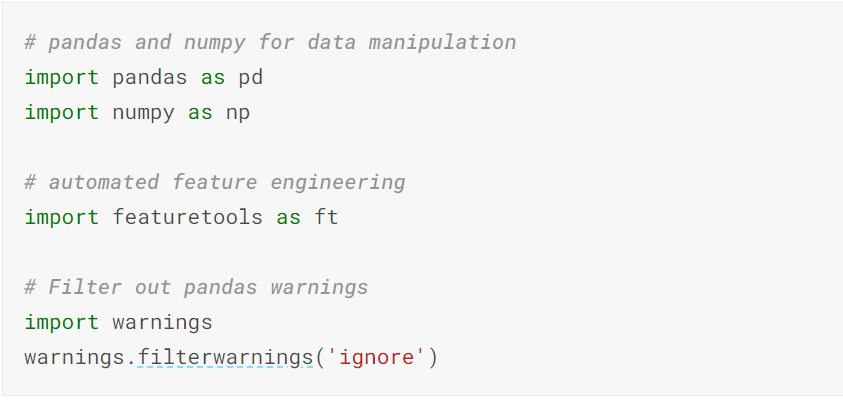
\includegraphics[scale=.8]{load1.png}
\clearpage %Page break
\subsubsection{Read in Data and Create Smaller Datasets}
We will limit the data to 1000 rows because automated feature engineering is computationally intensive work. Later we can refactor this code into functions and put it in a script to run on a more powerful machine.

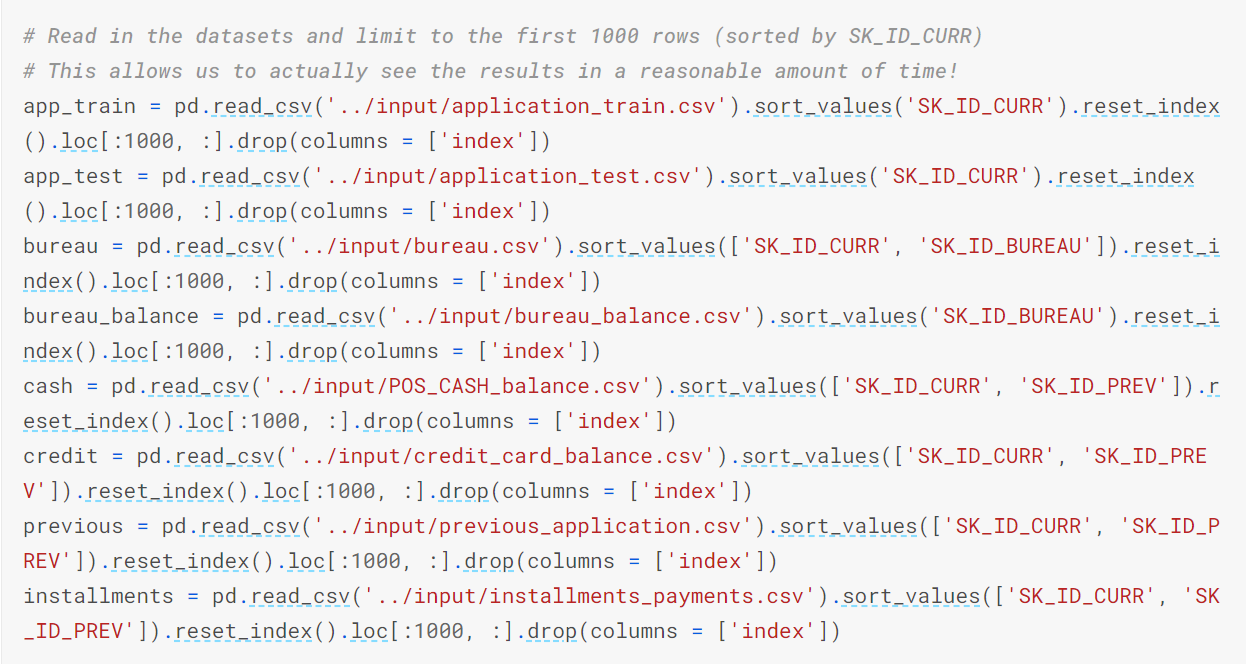
\includegraphics[scale=.8]{raedData.png}
\subsubsection{Properly Representing Variable Types}
There are a number of columns in the app dataframe that are represented as integers but are really discrete variables that can only take on a limited number of features. Some of these are Boolean flags (only 1 or 0) and two columns are ordinal (ordered discrete). To tell featuretools to treat these as Boolean variables, we need to pass in the correct datatype using a dictionary mapping {variable\_name: variable\_type}.

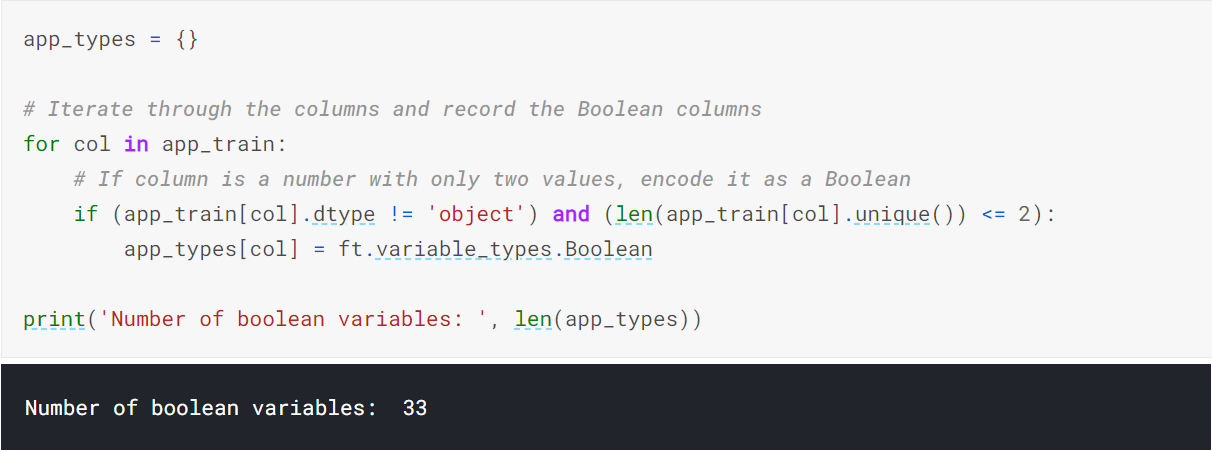
\includegraphics[scale=.8]{load3.png}
There are also two ordinal variables in the app data: the rating of the region with and without the city.
\clearpage %Page break
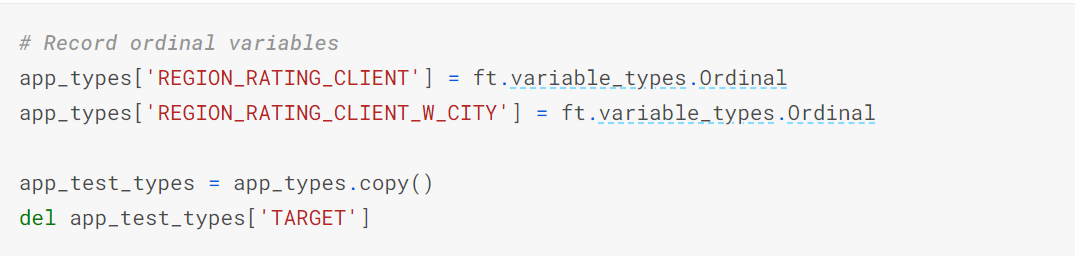
\includegraphics[scale=.8]{load4.png}

The previous data also has two Boolean variables.\\\\

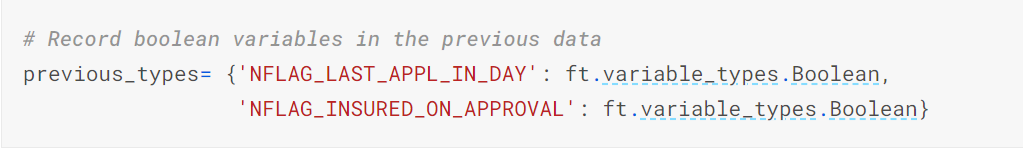
\includegraphics[scale=.8]{load 5.png}


\subsubsection{Time Variables}
Time can be a crucial factor in many datasets because behaviors change over time and therefore we want to make features to reflect this. For example, a client might be taking out larger and larger loans over time which could be an indicator that they are about to default or they could have a run of missed payments but then get back on track.

There are no explicit datetimes in the data, but there are relative time offsets. All the time offset are measured from the current application at Home Credit and are measured in months or days. For example, in bureau, the DAYS\_CREDIT column represents "How many days before current application did client apply for Credit Bureau credit". (Credit Bureau refers to any other credit organization besides Home Credit). Although we do not know the actual application date, if we assume a starting application date that is the same for all clients, then we can convert the MONTHS\_BALANCE into a datetime. This can then be treated as a relative time that we can use to find trends or identify the most recent value of a variable.
\paragraph{Replace Outliers}
There are a number of day offsets that are recorded as 365243. Reading through discussions, others replaced this number with np.nan. If we don't do this, Pandas will not be able to convert into a timedelta and throws an error that the number is too large.\\
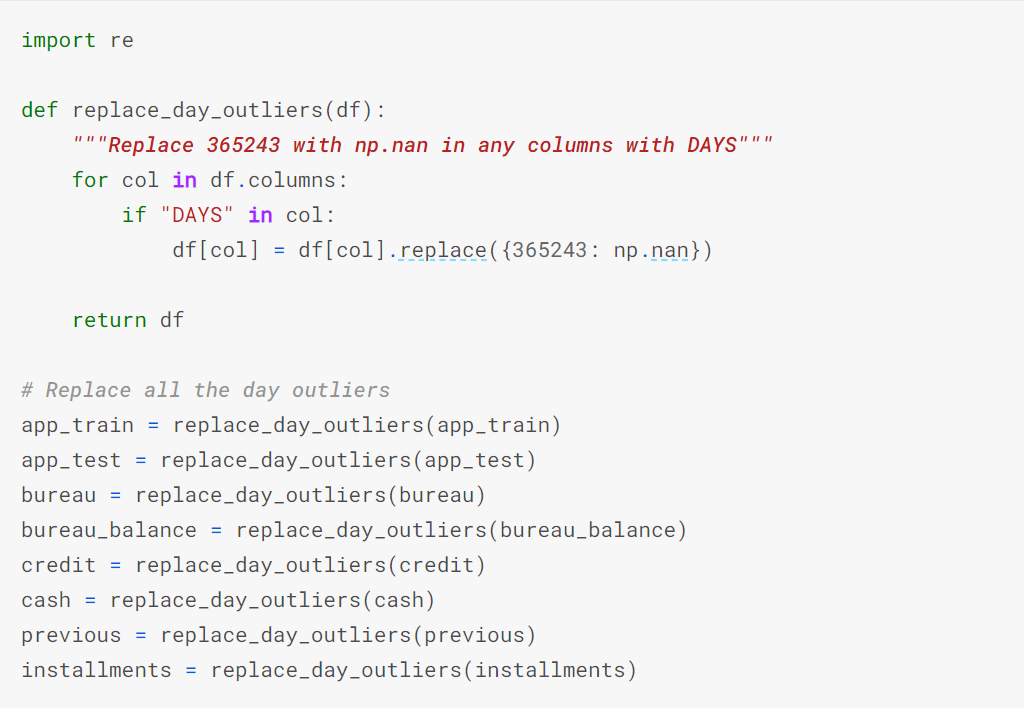
\includegraphics[scale=.8]{load6.png}
\\First we can establish an arbitrary date and then convert the time offset in months into a Pandas timedelta object.\\
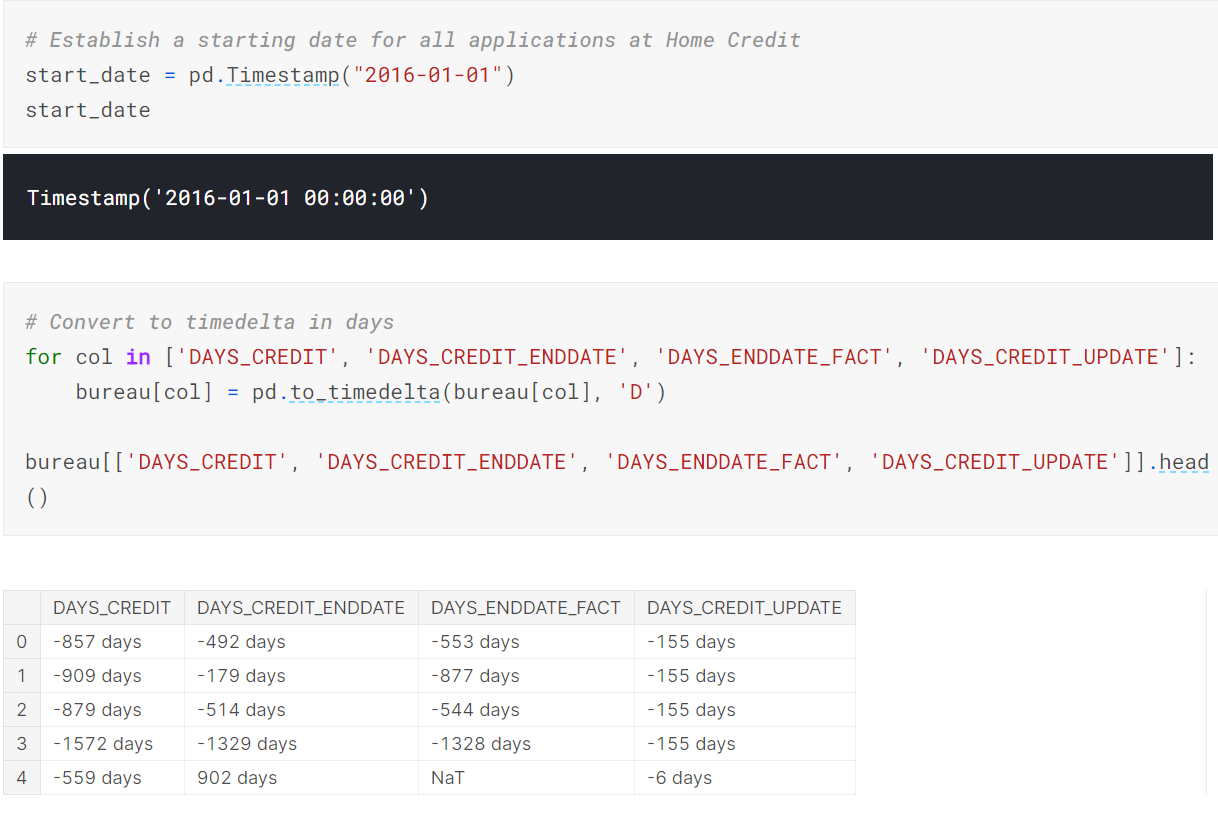
\includegraphics[scale=.8]{load7.png}
\\These four columns represent different offsets:\\




\begin{itemize}
 \item DAYS\_CREDIT: Number of days before current application at Home Credit client applied for loan at other financial institution. We will call this the application date, bureau\_credit\_application\_date and make it the time\_index of the entity.

 \item DAYS\_CREDIT\_ENDDATE: Number of days of credit remaining at time of client's application at Home Credit. We will call this the ending date, bureau\_credit\_end\_date

 \item DAYS\_ENDDATE\_FACT: For closed credits, the number of days before current application at Home Credit that credit at other financial institution ended.\\We will call this the closing date, bureau\_credit\_close\_date.

 \item DAYS\_CREDIT\_UPDATE: Number of days before current application at Home Credit that the most recent information about the previous credit arrived.\\We will call this the update date, bureau\_credit\_update\_date.\\
\end{itemize}
If we were doing manual feature engineering, we might want to create new columns such as by subtracting DAYS\_CREDIT\_ENDDATE from DAYS\_CREDIT to get the planned length of the loan in days, or subtracting DAYS\_CREDIT\_ENDDATE from DAYS\_ENDDATE\_FACT to find the number of days the client paid off the loan early. However, in this notebook we will not make any features by hand, but rather let featuretools develop useful features for us.\\\\To make date columns from the timedelta, we simply add the offset to the start date\\
 Create the date columns\\
bureau['bureau\_credit\_application\_date'] = start\_date + bureau['DAYS\_CREDIT']\\
bureau['bureau\_credit\_end\_date'] = start\_date + bureau['DAYS\_CREDIT\_ENDDATE']\\
bureau['bureau\_credit\_close\_date'] = start\_date + bureau['DAYS\_ENDDATE\_FACT']\\
bureau['bureau\_credit\_update\_date'] = start\_date + bureau['DAYS\_CREDIT\_UPDATE']\\
\paragraph{Plot for a sanity check}
To make sure the conversion went as planned, let's make a plot showing the distribution of loan lengths\\
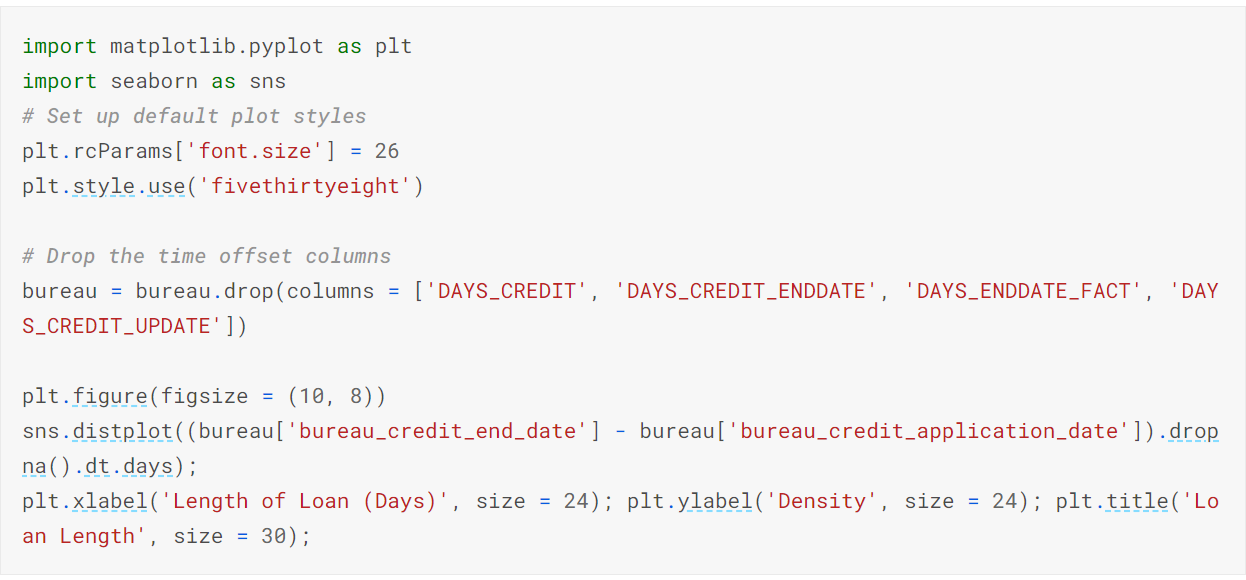
\includegraphics[scale=.8]{load8.png}
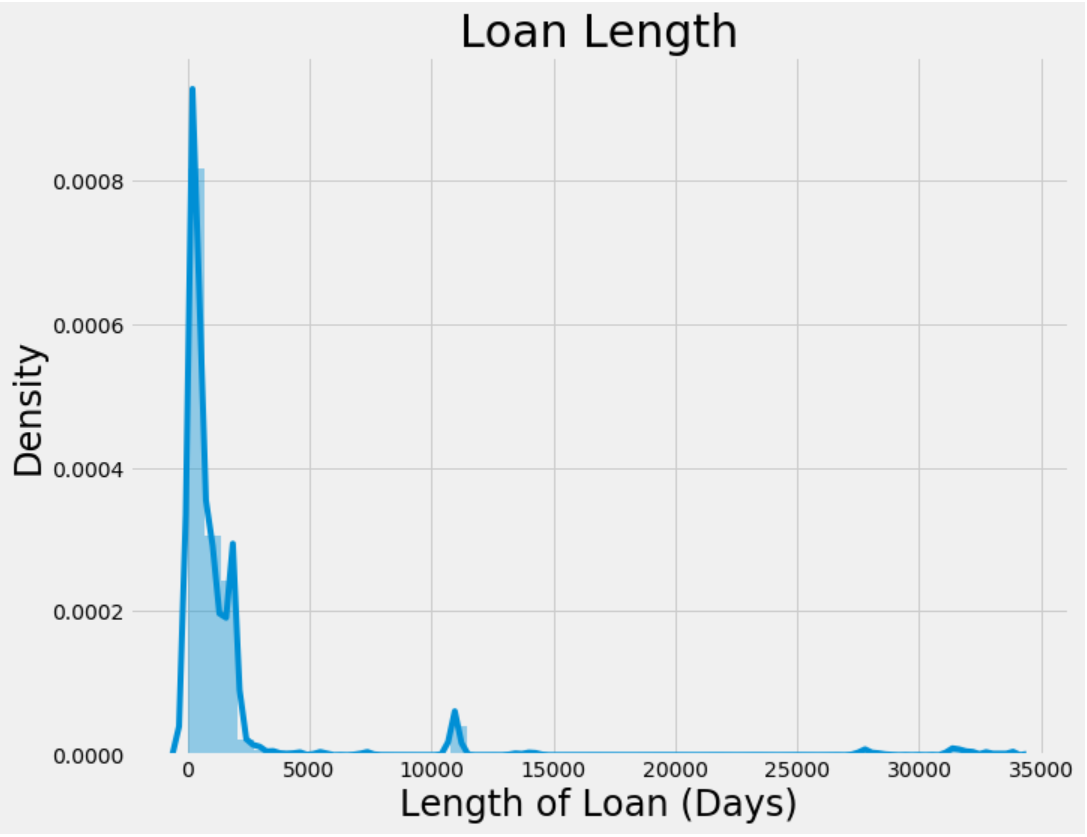
\includegraphics[scale=.8]{load9.png}
\\\\It looks as if there are a number of loans that are unreasonably long. Reading through the discussions, other people had noticed this as well. At this point, we will just leave in the outliers. We also will drop the time offset columns.\\\\
\paragraph{Bureau Balance}
The bureau balance dataframe has a MONTHS\_BALANCE column that we can use as a months offset. The resulting column of dates can be used as a time\_index.\\
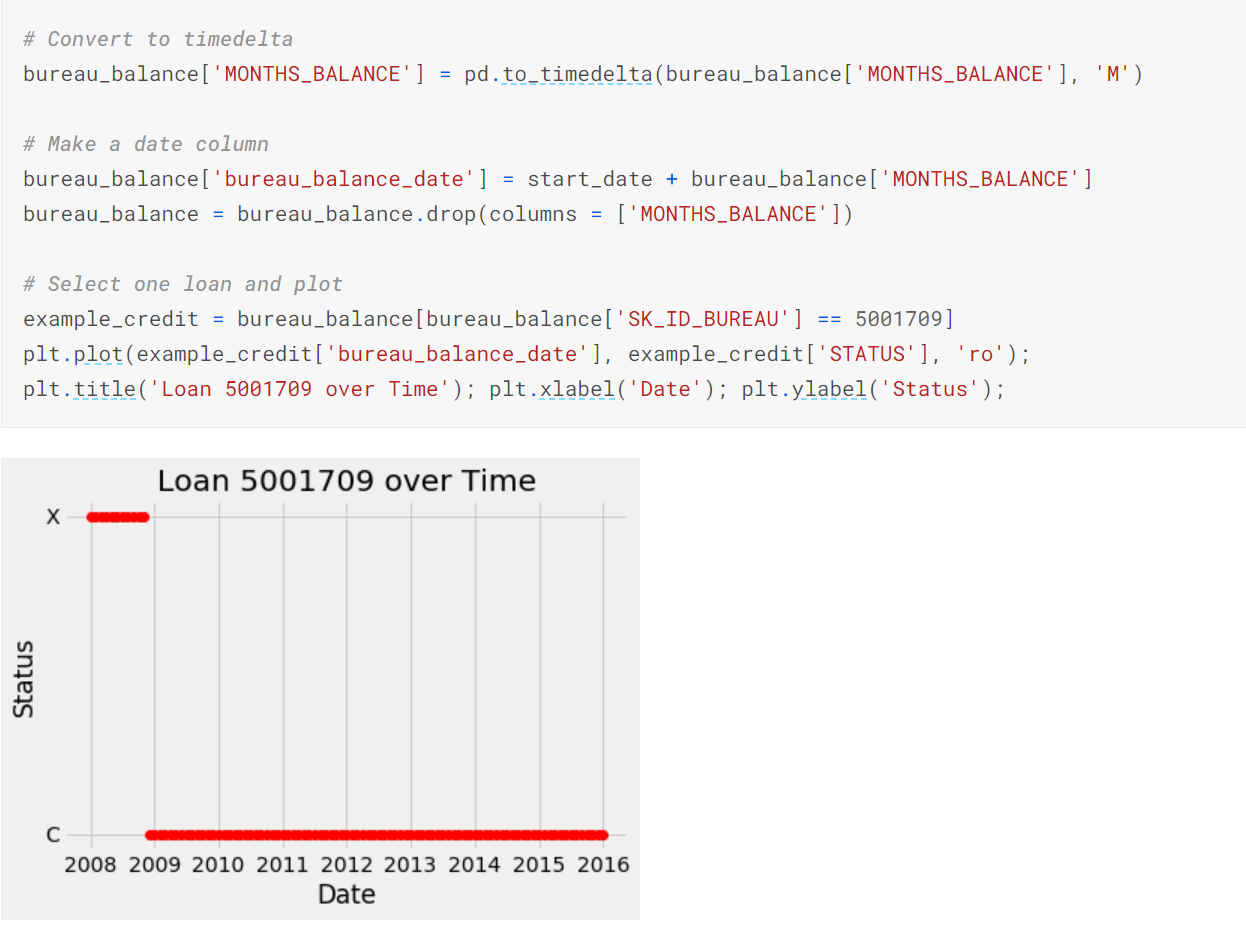
\includegraphics[scale=.8]{load10.png}
\paragraph{Previous Applications}
The previous dataframe holds previous applications at Home Credit. There are a number of time offset columns in this dataset:\\
\begin{itemize}
 \item  DAYS\_DECISION: number of days before current application at Home Credit that decision was made about previous application. This will be the time\_index of the data.
 \item DAYS\_FIRST\_DRAWING: number of days before current application at Home Credit that first disbursement was made
 \item DAYS\_FIRST\_DUE: number of days before current application at Home Credit that first due was suppoed to be
 \item DAYS\_LAST\_DUE\_1ST\_VERSION: number of days before current application at Home Credit that first was??
 \item DAYS\_LAST\_DUE: number of days before current application at Home Credit of last due date of previous application
 \item DAYS\_TERMINATION: number of days before current application at Home Credit of expected termination
\end{itemize}
Let's convert all these into timedeltas in a loop and then make time columns.\\
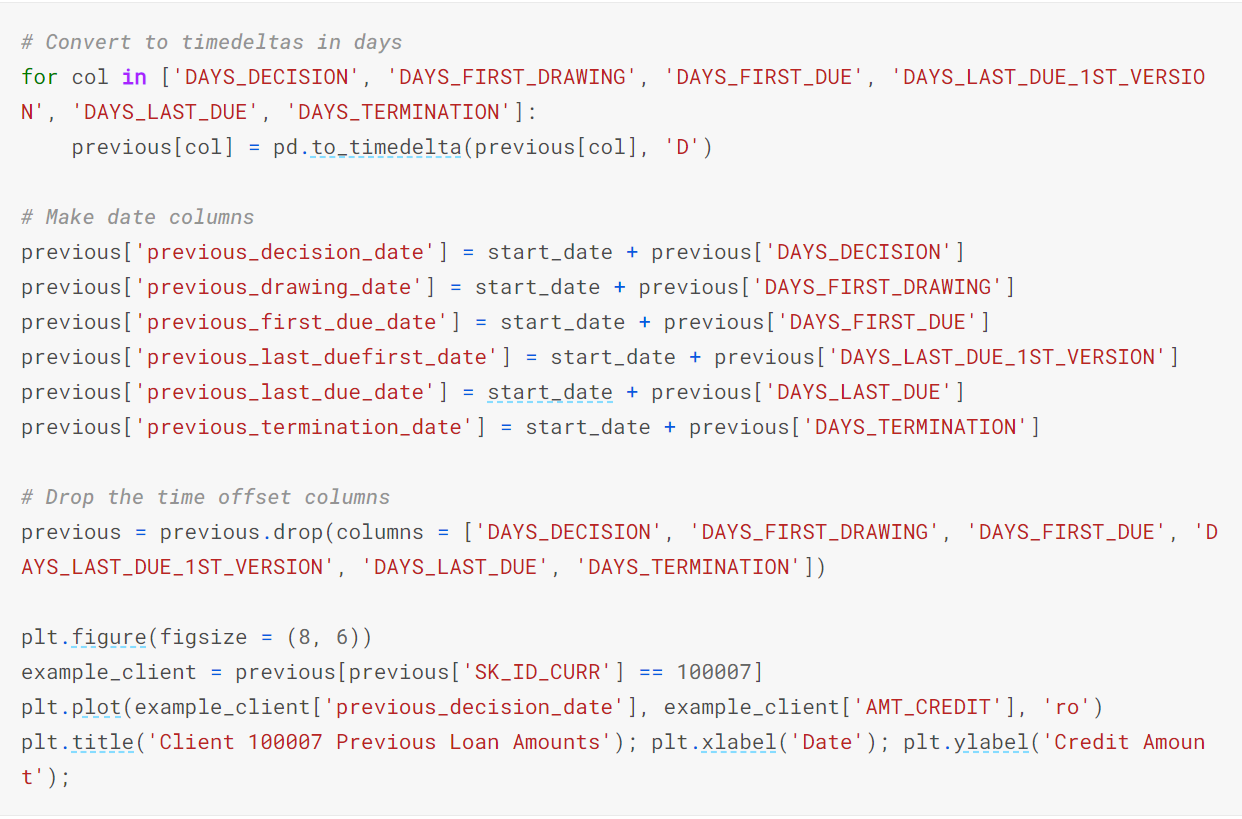
\includegraphics[scale=.8]{load11.png}
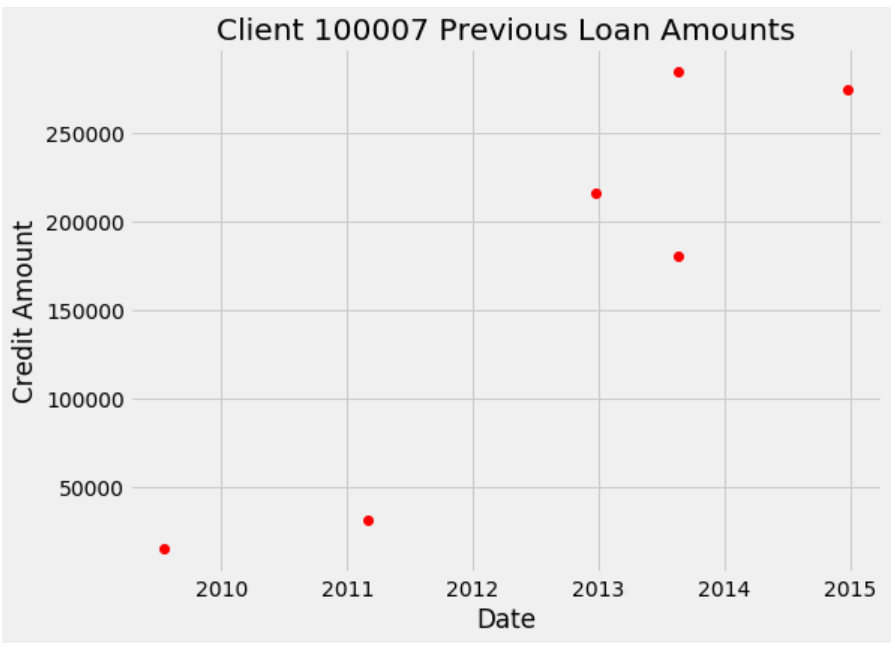
\includegraphics[scale=.8]{load12.png}
\paragraph{Previous Credit and Cash}
The credit\_card\_balance and POS\_CASH\_balance each have a MONTHS\_BALANCE column with the month offset. This is the number of months before the current application at Home Credit of the previous application record. These will represent the time\_index of the data.\\
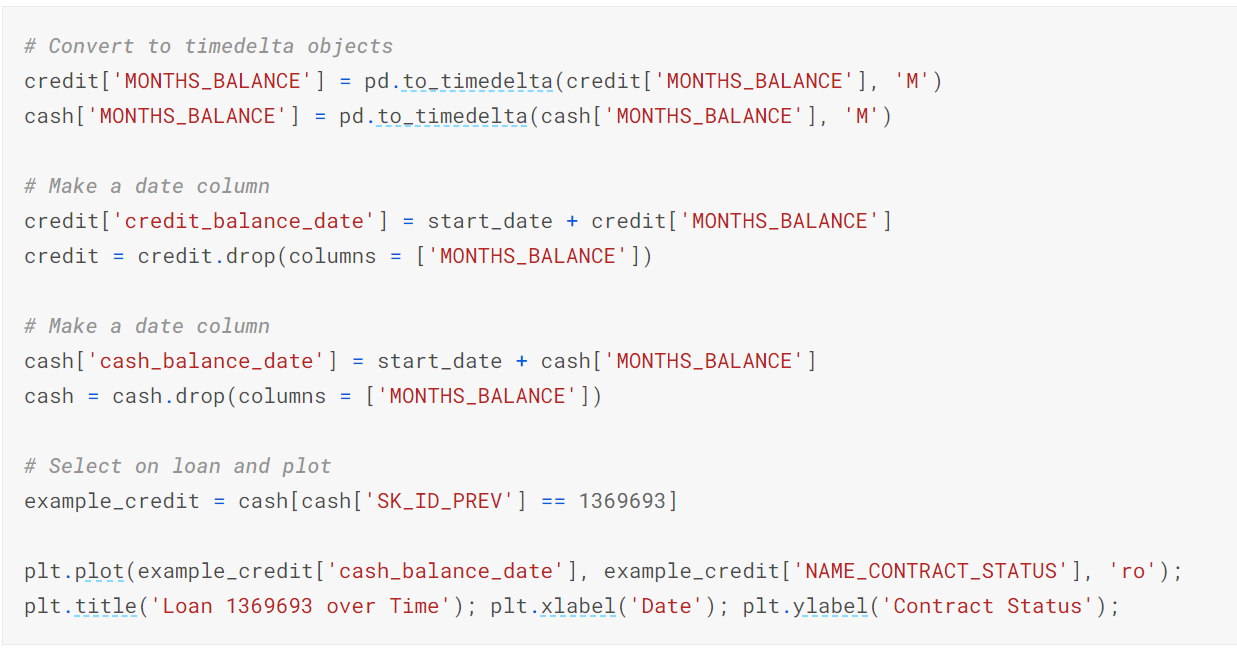
\includegraphics[scale=.8]{13.png}
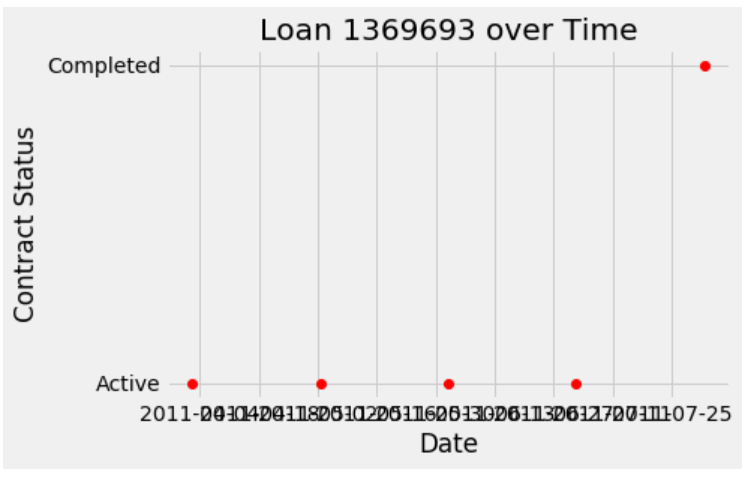
\includegraphics[scale=.8]{14.png}
\paragraph{Installments Payments}
The installments\_payments data contains information on each payment made on the previous loans at Home Credit. It has two date offset columns:
\begin{itemize}
 \item DAYS\_INSTALMENT: number of days before current application at Home Credit that previous installment was supposed to be paid
 \item DAYS\_ENTRY\_PAYMENT: number of days before current application at Home Credit that previous installment was actually paid
\end{itemize}
By now the process should be familiar: convert to timedeltas and then make time columns. The DAYS\_INSTALMENT will serve as the time\_index.\\
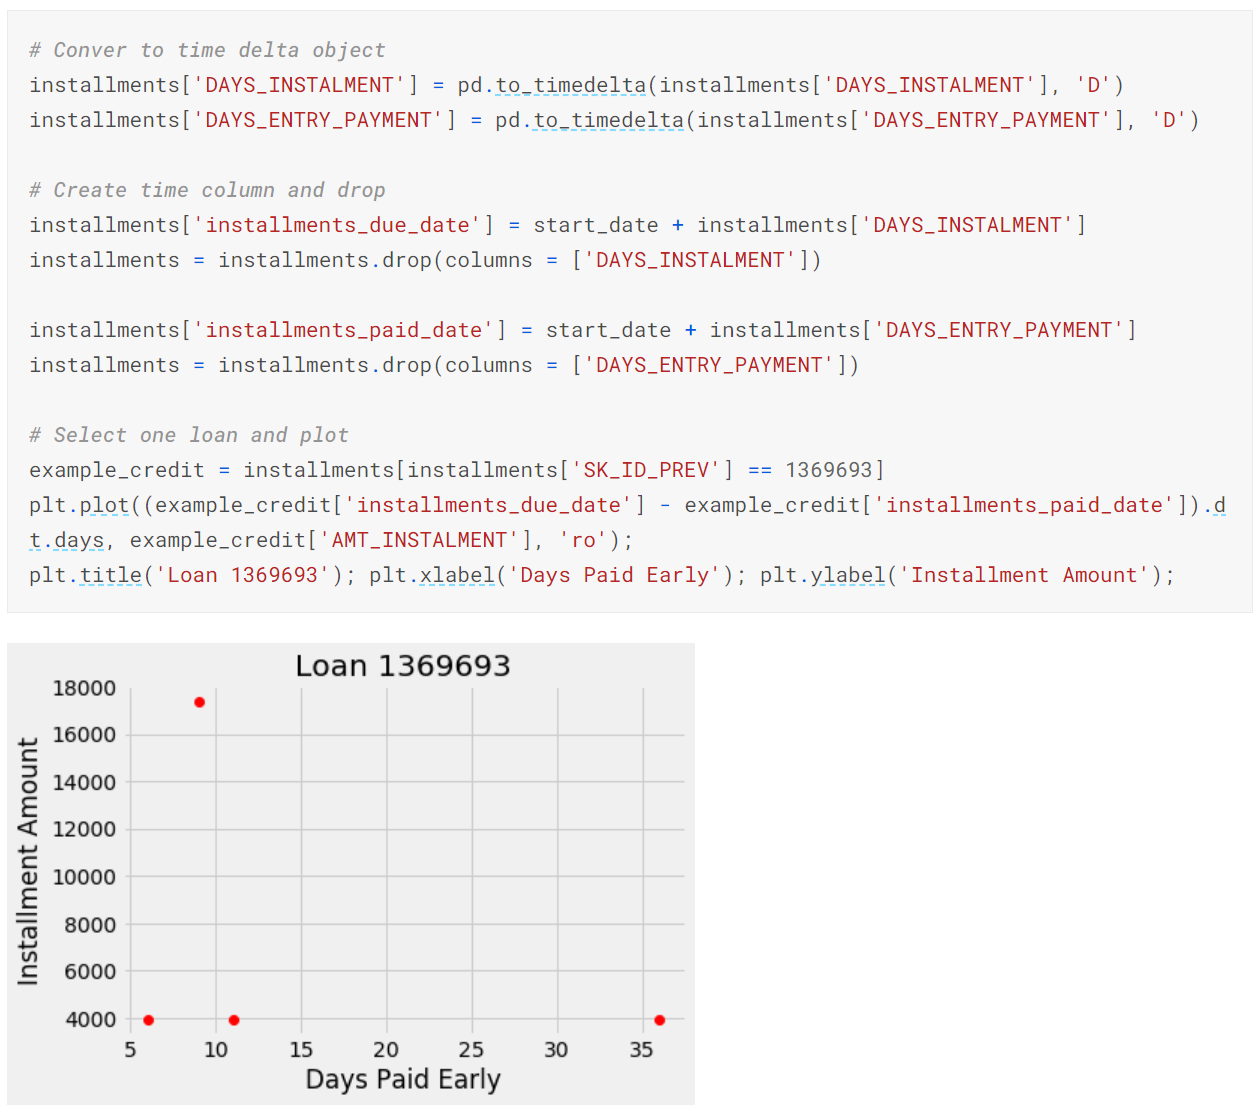
\includegraphics[scale=.8]{15.png}
\subsubsection{Applying Featuretools}
We can now start making features using the time columns. We will create an entityset named clients much as before, but now we have time variables that we can use.\\
\#Make an entityset\\
es = ft.EntitySet(id = 'clients')\\
\paragraph{Entities}
When creating the entities, we specify the index, the time\_index (if present), and the variable\_types (if they need to be specified).\\
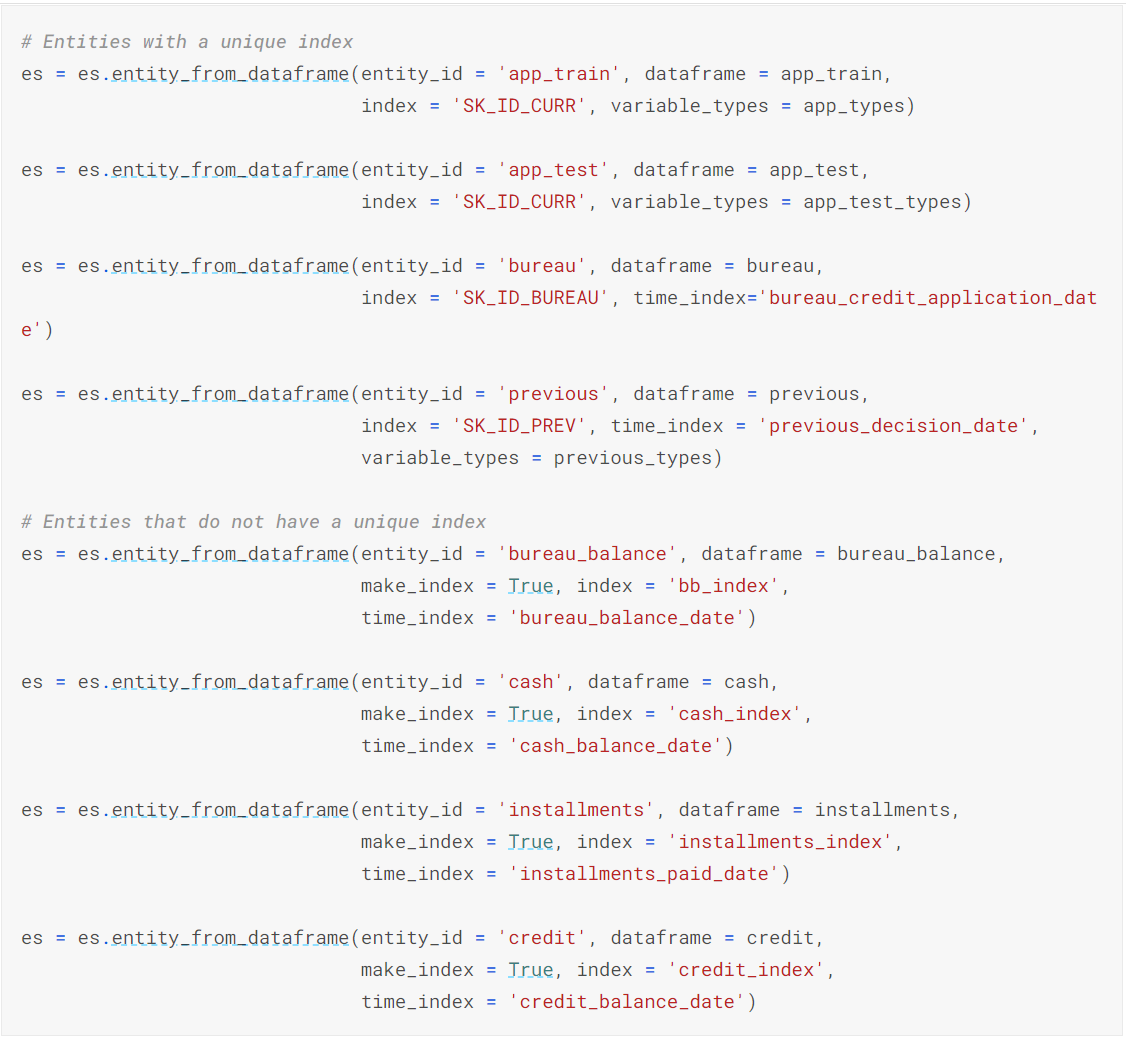
\includegraphics[scale=.8]{16.png}
\subsubsection{Relationships}
Not surprisingly, the relationships between tables has not changed since the previous implementation.\\
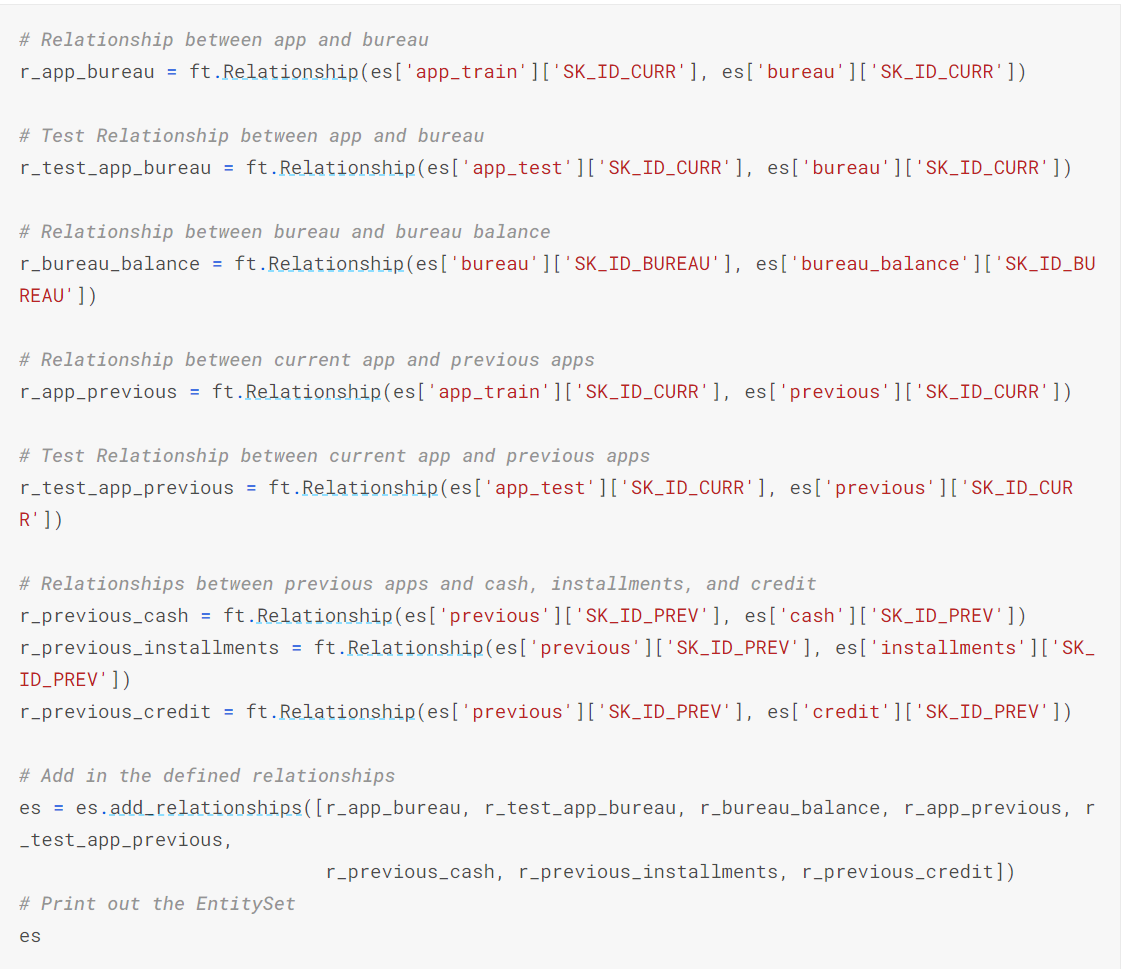
\includegraphics[scale=.7]{17.png}\\
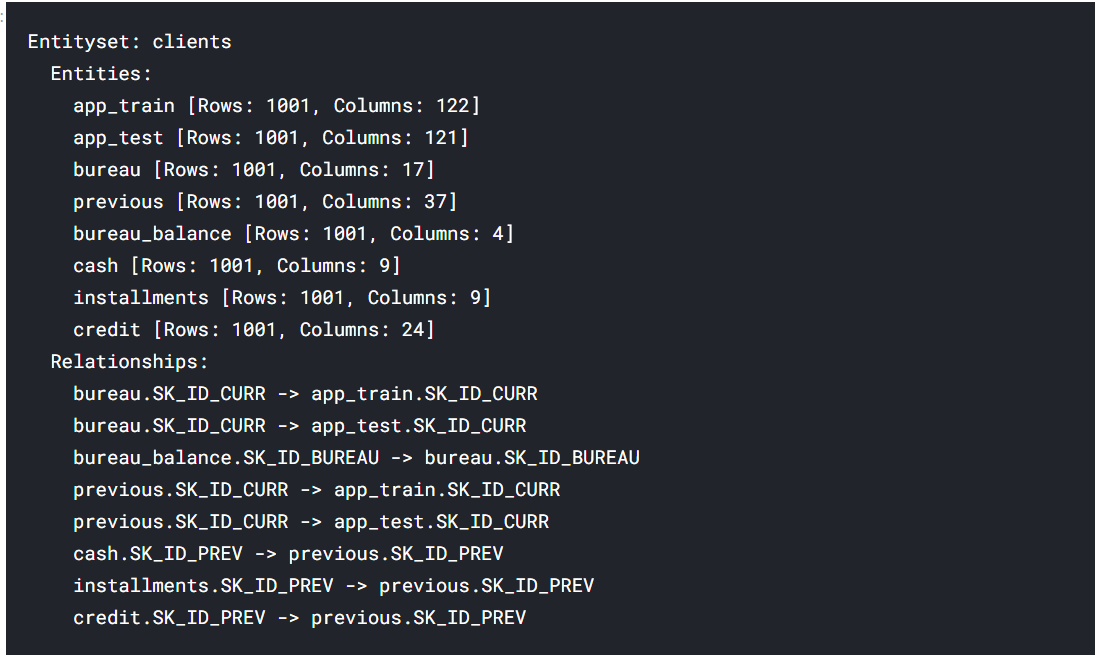
\includegraphics[scale=.7]{18.png}
\subsubsection{Time Features}
Let's look at some of the time features we can make from the new time variables. Because these times are relative and not absolute, we are only interested in values that show change over time, such as trend or cumulative sum. We would not want to calculate values like the year or month since we choose an arbitrary starting date.

Throughout this notebook, we will pass in a chunk\_size to the dfs call which specifies the number of rows (if an integer) or the fraction or rows to use in each chunk (if a float). This can help to optimize the dfs procedure, and the chunk\_size can have a significant effect on the run time. Here we will use a chunk size equal to the number of rows in the data so all the results will be calculated in one pass. We also want to avoid making any features with the testing data, so we pass in ignore\_entities = [app\_test].\\
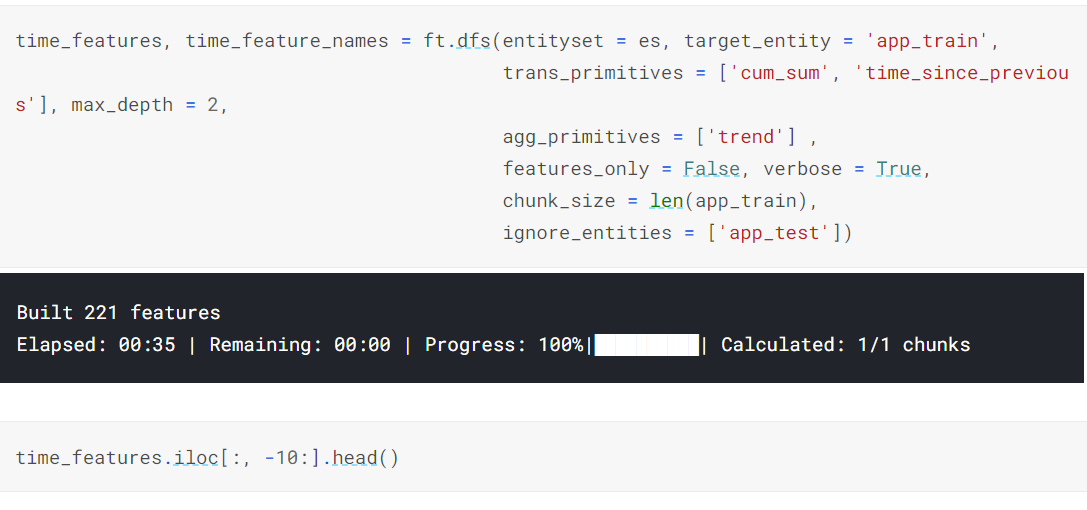
\includegraphics[scale=.7]{19.png}\\
Let's visualize one of these new variables. We can look at the trend in credit size over time. A positive value indicates that the loan size for the client is increasing over time\\
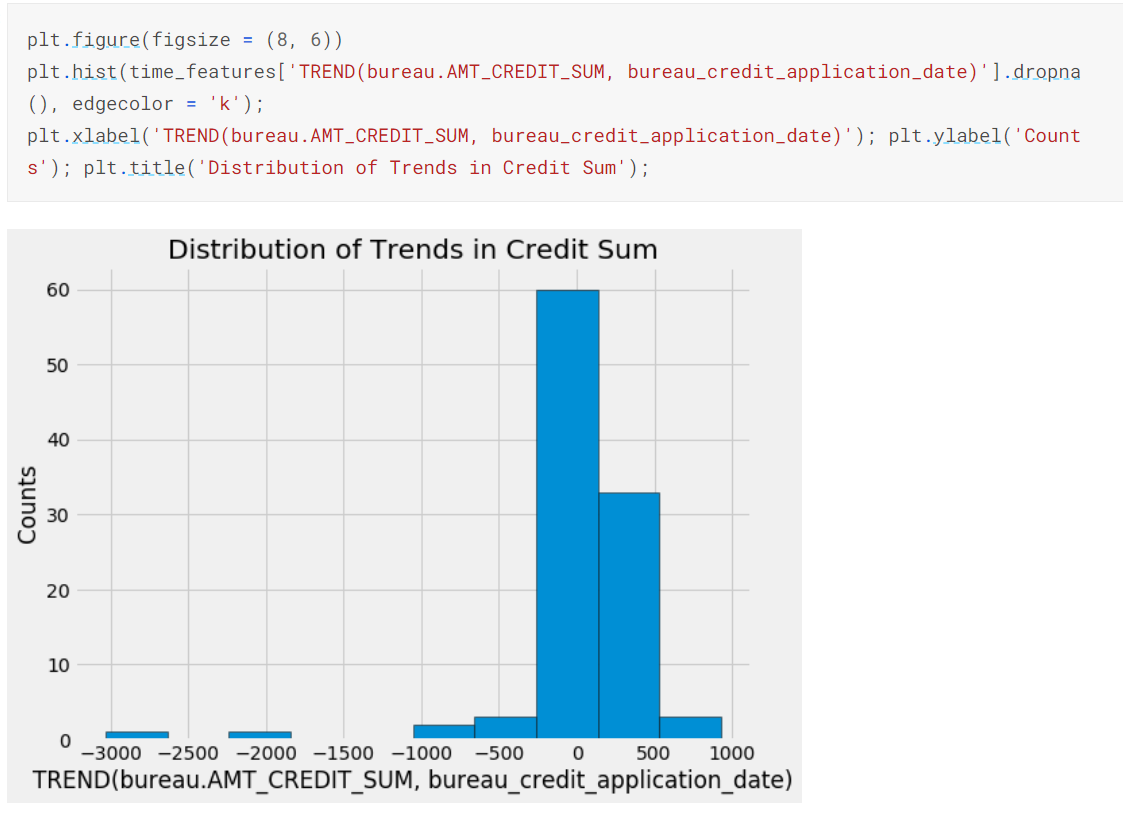
\includegraphics[scale=.7]{20.png}\\
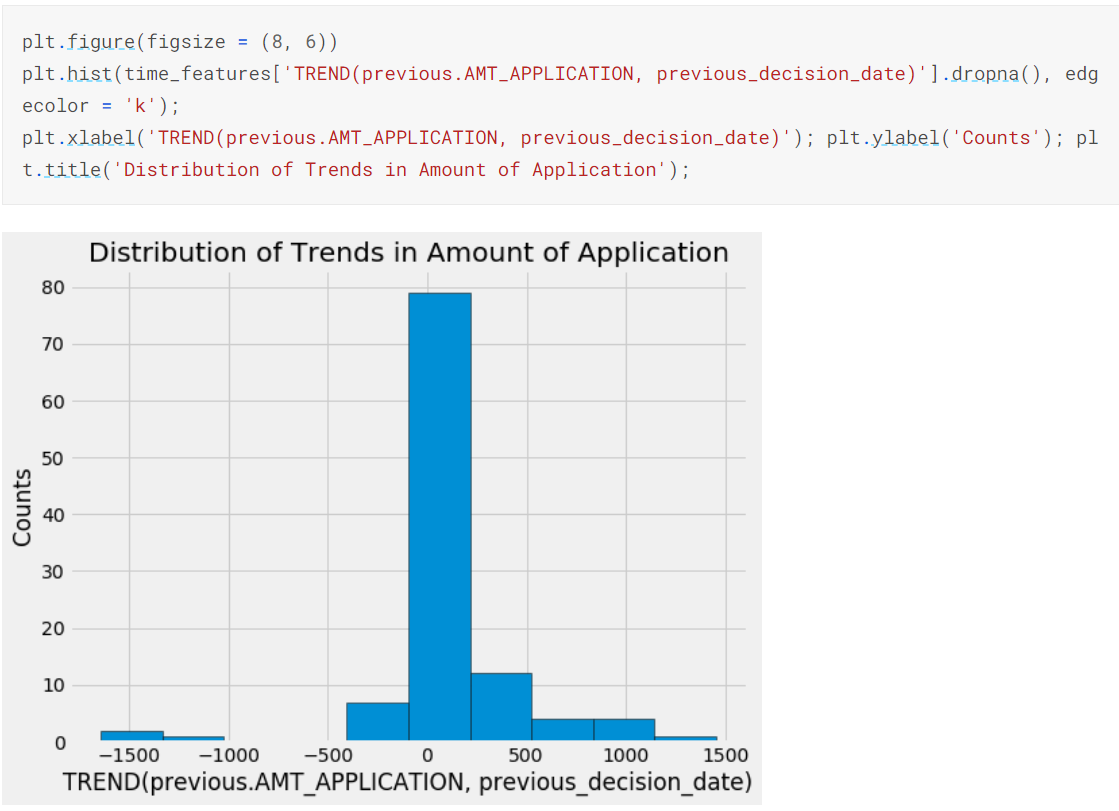
\includegraphics[scale=.7]{21.png}\\
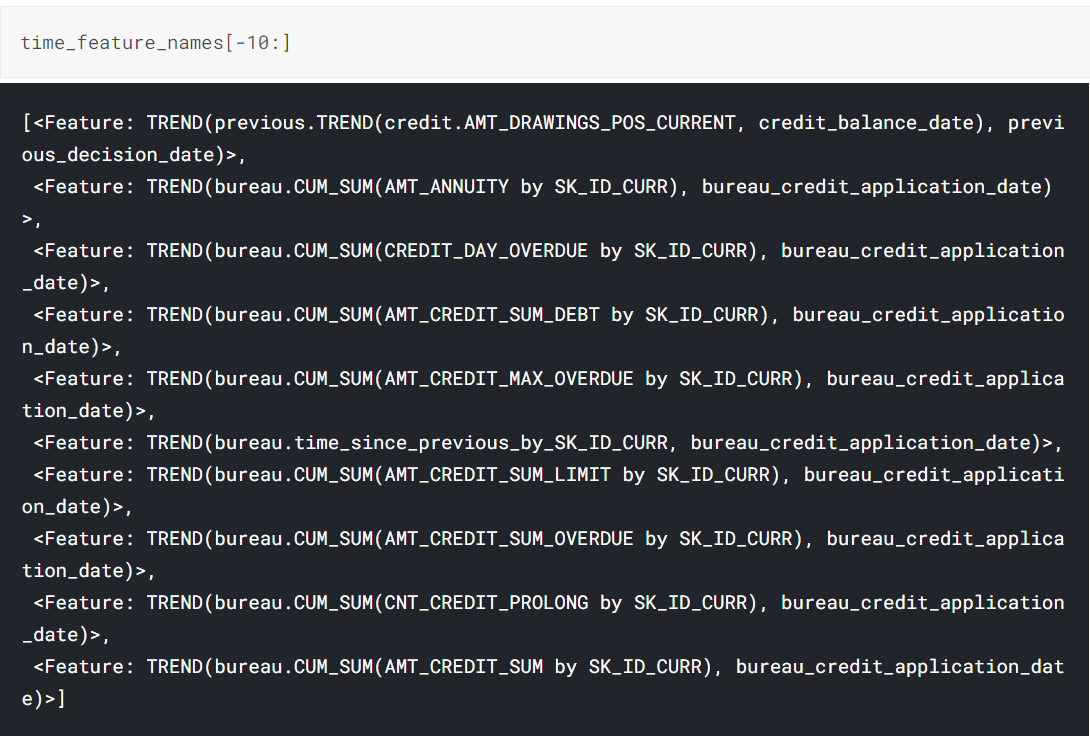
\includegraphics[scale=.7]{22.png}
\subsubsection{Interesting Values}
Another method we can use in featuretools is "interesting values." Specifying interesting values will calculate new features conditioned on values of existing features. For example, we can create new features that are conditioned on the value of NAME\_CONTRACT\_STATUS in the previous dataframe. Each stat will be calculated for the specified interesting values which can be useful when we know that there are certain indicators that are of greater importance in the data.\\
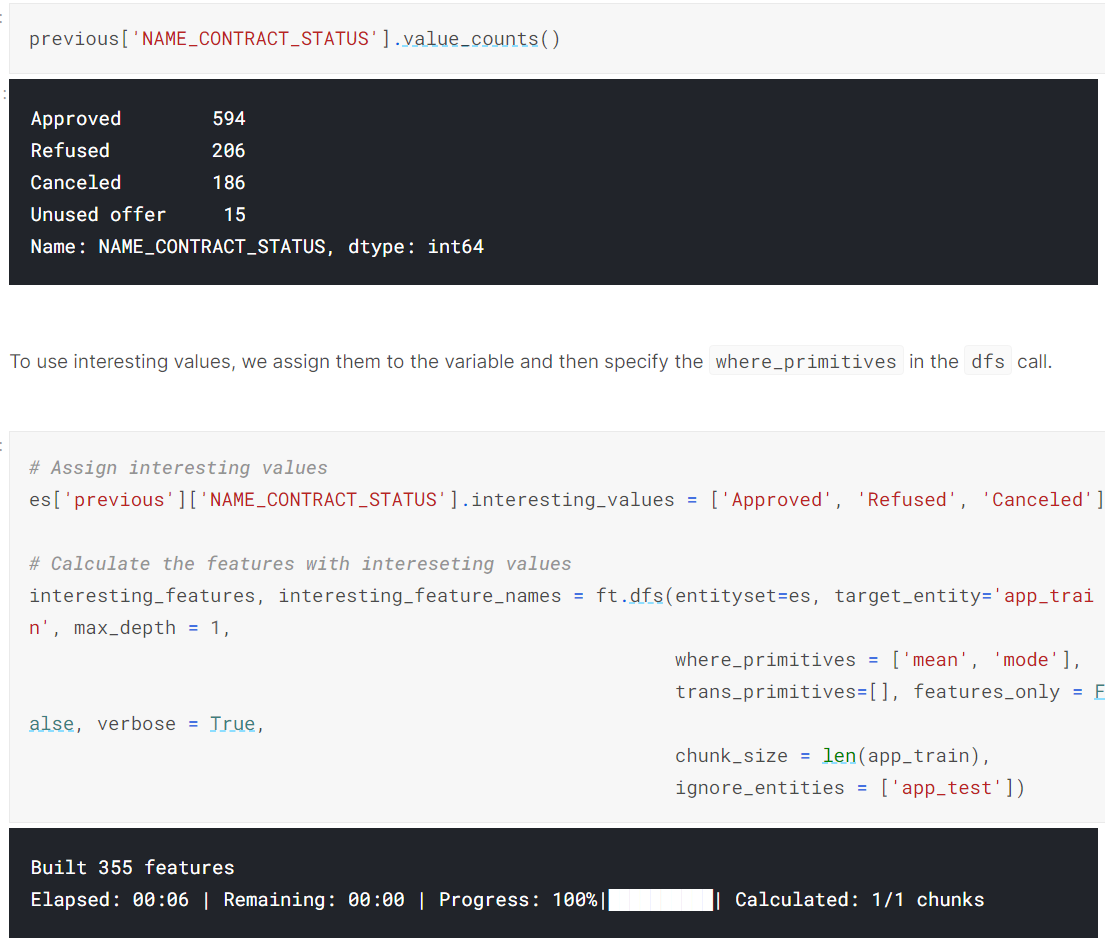
\includegraphics[scale=.8]{23.png}\\\\''
One of the features is MEAN(previous.CNT\_PAYMENT WHERE NAME\_CONTRACT\_STATUS = Approved). This shows the average "term of previous credit" on previous loans conditioned on the previous loan being approved. We can compare the distribution of this feature to the MEAN(previous.CNT\_PAYMENT WHERE NAME\_CONTRACT\_STATUS = Canceled) to see how these loans differ.\\
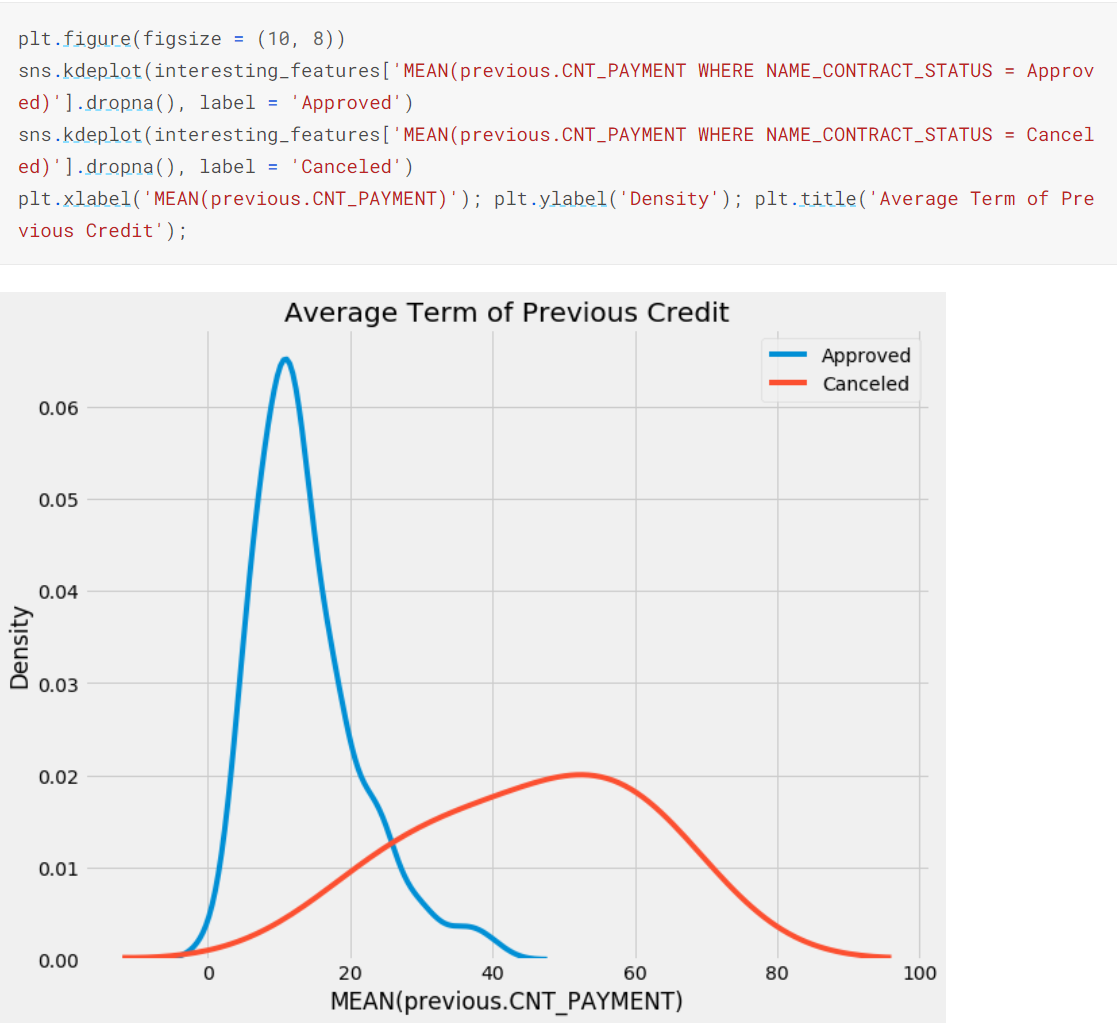
\includegraphics[scale=.8]{24.png}\\
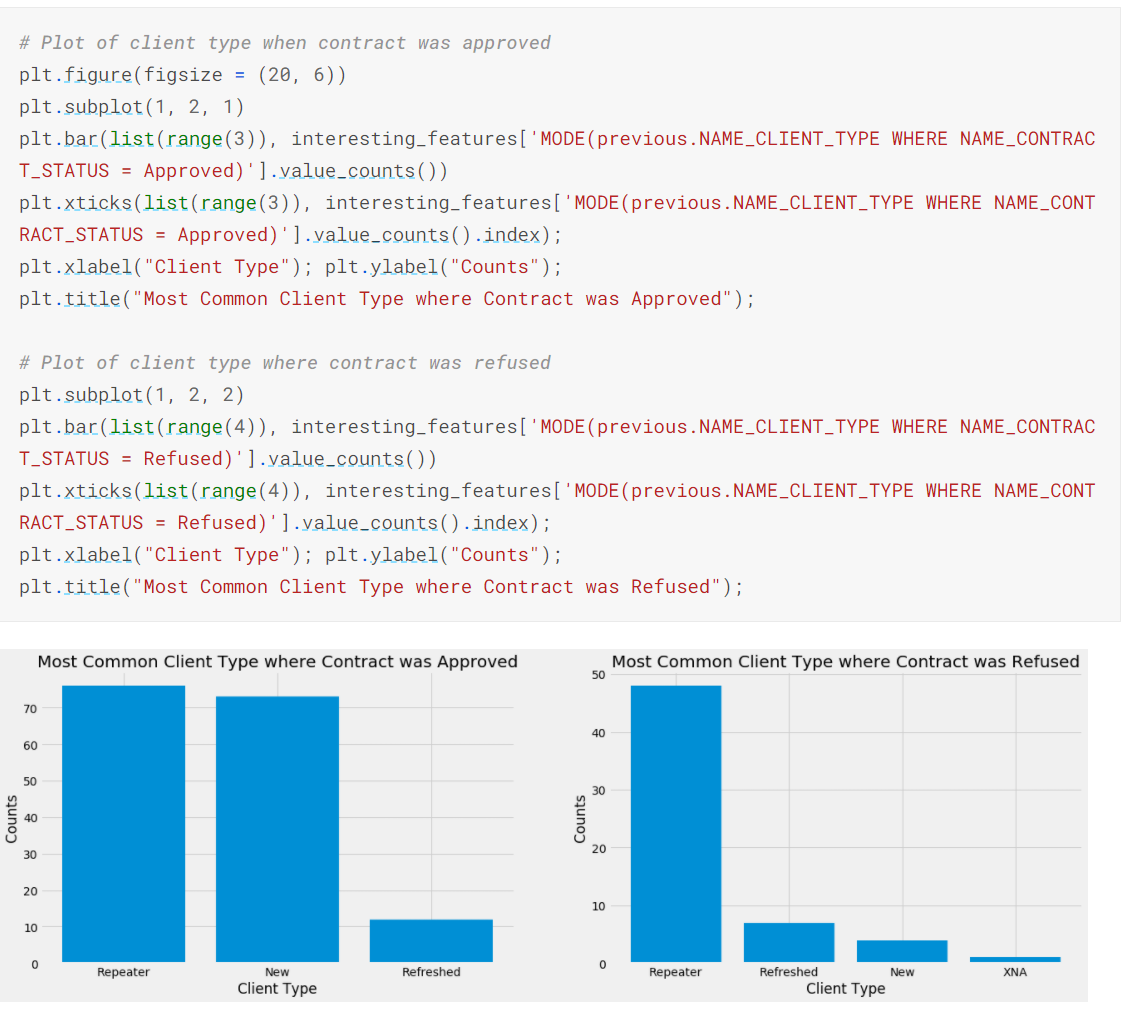
\includegraphics[scale=.8]{25.png}\\
Based on the most important features returned by a model, we can create new interesting features. This is one area where we can apply domain knowledge to feature creation.

\subsubsection{Seed Features}
An additional extension to the default aggregations and transformations is to use seed features. These are user defined features that we provide to deep feature synthesis that can then be built on top of where possible.

As an example, we can create a seed feature that determines whether or not a payment was late. This time when we make the dfs function call, we need to pass in the seed\_features argument.\\
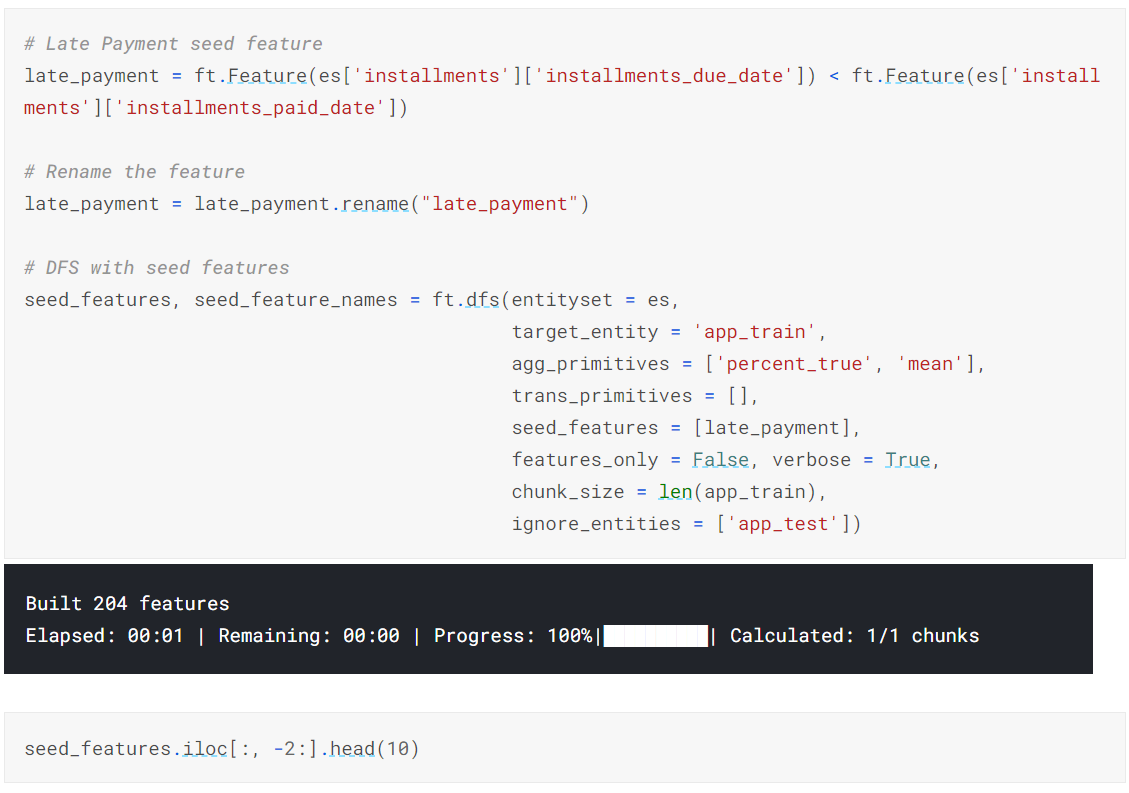
\includegraphics[scale=.7]{26.png}\\
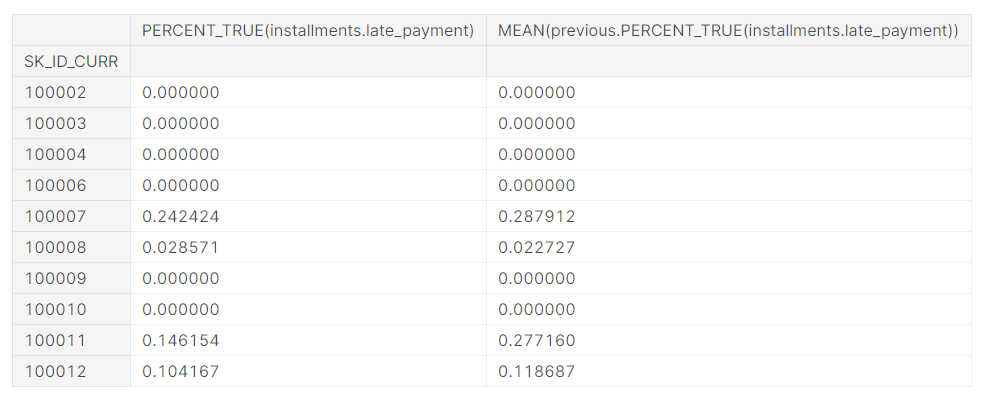
\includegraphics[scale=.8]{27.png}\\
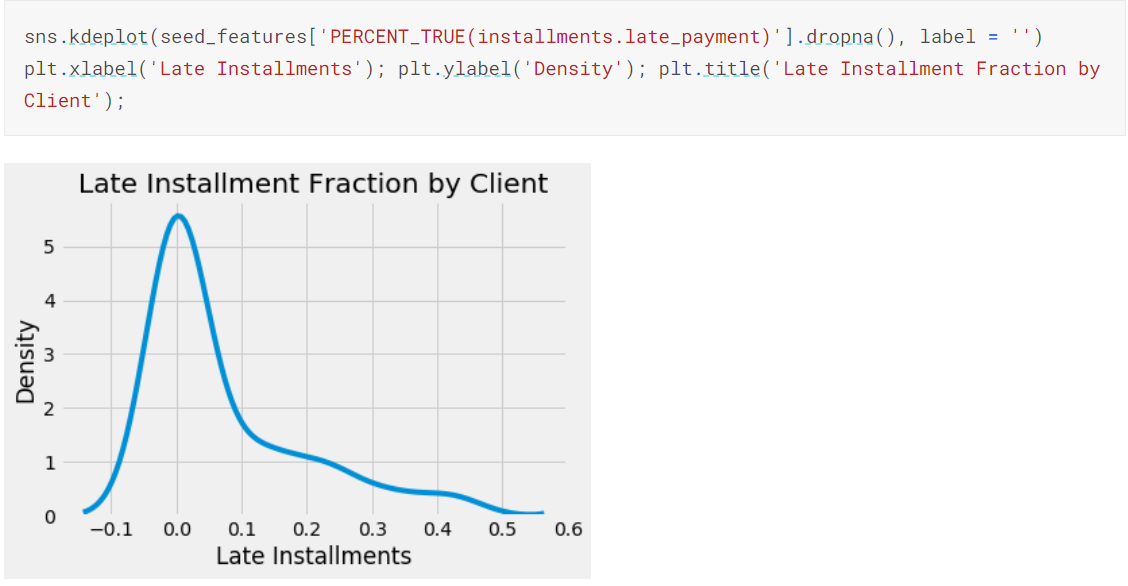
\includegraphics[scale=.7]{28.png}\\


\subsubsection{Putting it all Together}
Finally, we can run deep feature synthesis with the time variables, with the correct specified categorical variables, with the interesting features, with the seed features, and with the custom features. To actually run this on the entire dataset, we can take the code here, put it in a script, and then use more computational resources.\\
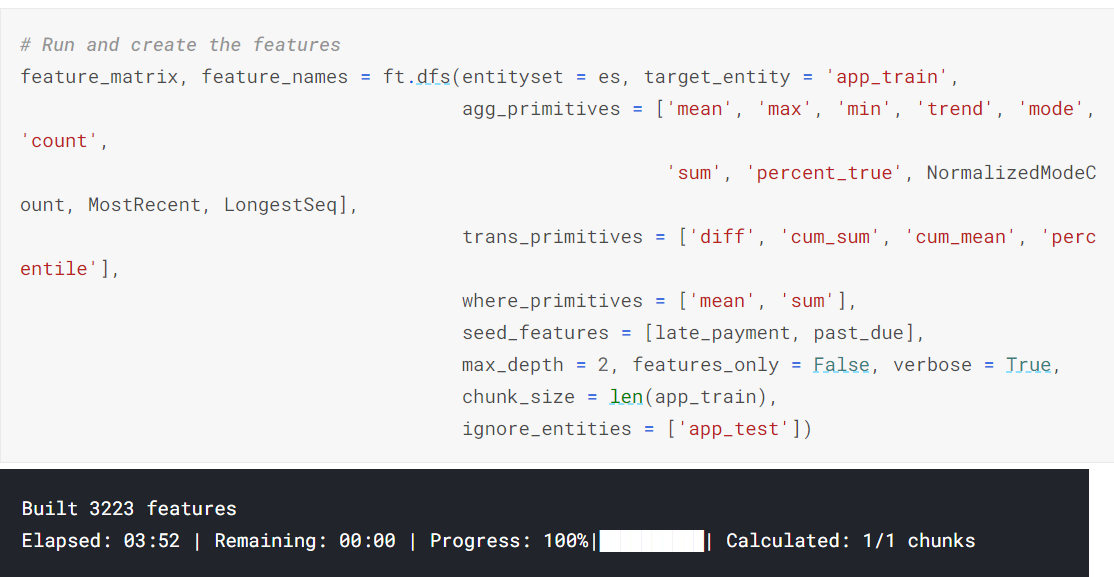
\includegraphics[scale=.7]{29.png}\\
We will now do the same operation applied to the test set. Doing the calculations separately should prevent leakage from the testing data into the training data.\\
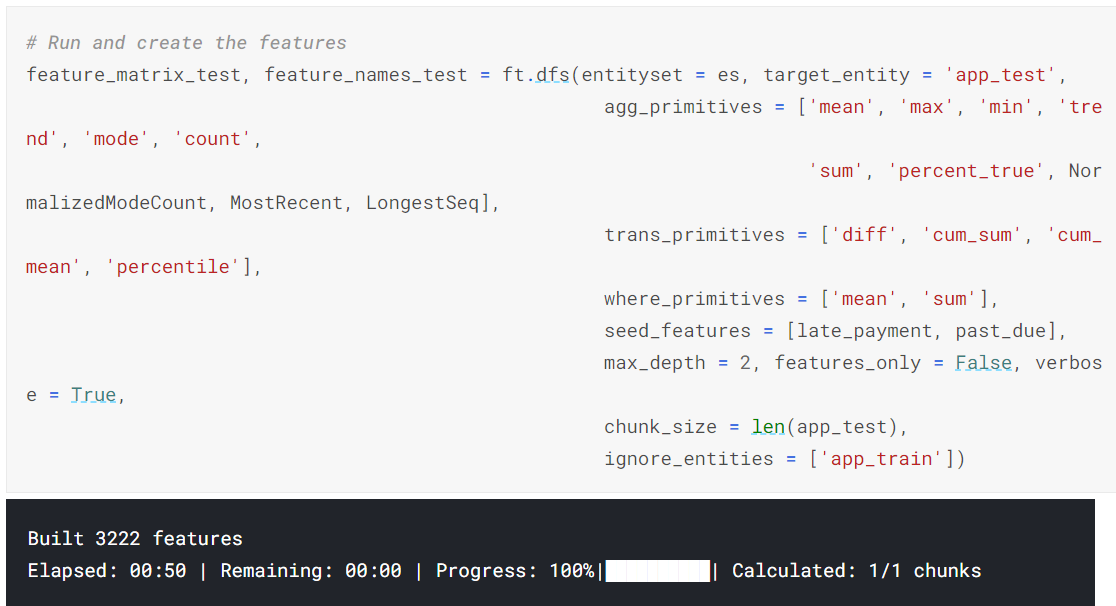
\includegraphics[scale=.7]{30.png}\\
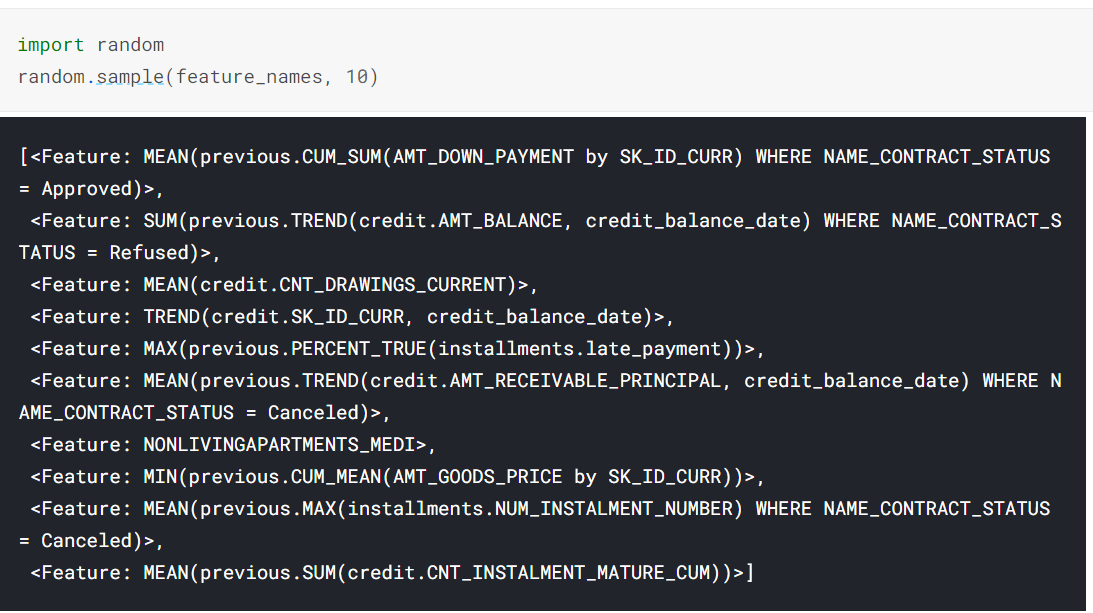
\includegraphics[scale=.7]{31.png}\\
\subsubsection{Conclusion}
 we explored some of the advanced functionality in featuretools including:

Time Variables: allow us to track trends over time
Interesting Variables: condition new features on values of existing features
Seed Features: define new features manually that featuretools will then build on top of
Custom feature primitives: design any transformation or aggregation feature that can incorporate domain knowledge
We can use these methods to encode domain knowledge about a problem into our features or create features based on what others have found useful. The next step from here would be to run the script on the entire dataset, then use the features for modeling. We could use the feature importances from the model to determine the most relevant features, perform feature selection, and then go through another round of feature synthesis with a new set of of primitives, seed features, and interesting features. As with many aspects of machine learning, feature creation is largely an empirical and iterative procedure.

\subsection{Home Credit Default Report 2}

\subsubsection{Objective}
The main objective is to identify the potential Defaulters based on the given data about the applicants.\\
The probability of classification is essential because we want to be very sure when we classify someone as a Non-Defaulter, as the cost of making a mistake can be very high to the company.
\subsubsection{Metric}
 ROC-AUC Score:This metric is insensitive to class imbalance. It works by ranking the probabilities of prediction of the positive class label and calculating the Area under the ROC Curve which is plotted between True Positive Rates and False Positive Rates for each threshold value.\\\\
 Recall Score: It is the ratio of the True Positives predicted by the model and the total number of Actual Positives. It is also known as True Positive Rate.\\\\
 Precision Score: It is the ratio of True Positives and the Total Positives predicted by the model.
\\\\
 Confusion Matrix : The confusion matrix helps us to visualize the mistakes made by the model on each of the classes, be it positive or negative. Hence, it tells us about misclassifications for both classes.
\\
\subsubsection{Dataset Description}
The dataset provided contains lots of details about the borrower. It is segregated into multiple relational tables, which contain applicants’ static data such as their gender, age, number of family members, occupation, and other related fields, applicant’s previous credit history obtained from the credit bureau department, and the applicant’s past credit history within the Home Credit Group itself. The dataset is an imbalanced dataset, where the Negative class dominates the Positive class, as there are only a few number of defaulters among all the applicants.
\subsubsection{Exploratory Data Analysis}
We will first start by checking the shapes of the tables in hand. Since there are 8 tables in total, we will load each table, and print their shapes and a few of their rows.\\
We also found that all the tables contain large number of missing values, and thus it is important to address the counts of the missing values. We have plotted Bar Plots for the missing values of each column for each table.
\subsubsection{Distribution of Target Variable}

Now, let us have a look at the distribution of the Target Variable in our Training Dataset. We see that there are only 8\% (24.8k) Defaulters, and 91.9\% (282.6k) Non-Defaulters in the train dataset. This shows that the Positive class is a minority class in our dataset. It also implies that it is an Imbalanced Dataset, and we need to come up with adequate ways to handle it.

\subsubsection{Column Types}
Let's look at the number of columns of each data type.  float64= 65,int64=41,object= 16,dtype= int64
\subsubsection{Analysis of Continuous Variables}

For continuous variables, we have used Box-Plots, Violin-Plots, and PDFs extensively. We have plotted the distribution of data-points for both Defaulters and Non-Defaulters together, and try to see if these distributions are similar or distinguishable.
Similar to code for plotting categorical variables, we have generalized the code for continuous variables as well.

\subsubsection{Algorithm}
Logistic Regression \\
Random Forest
\subsubsection{Model Interpretation}
\subsubsection{Conclusion}
We also noticed some correlated features from the correlation analysis, which would be increasing the dimensionality of data without adding much value. We would ideally want to remove such features, provided they don’t degrade the performance of the model.
The dataset is imbalanced, and we would need to come up with techniques to handle it.
For Default Risk prediction, the Defaulters usually tend to have some behavior which deviate from the normal, and thus, we cannot remove outliers or far-off points, as they may suggest some important Defaulting tendency.
With all these observations and insights in mind, we will move to the Data Cleaning and Feature Engineering task.

%----------------------------------------------------------------------------------------
%	REFERENCE LIST
%----------------------------------------------------------------------------------------

\begin{thebibliography}{99} % Bibliography - this is intentionally simple in this template

\bibitem{discussionlightgbm}
Abdelwahed Assklou and Aguiar.
\newblock \href{https://www.kaggle.com/c/home-credit-default-risk/discussion/64580}{7th solution - **Not great things but small things in a great way.**}
\newblock {\em Kaggle}.

\bibitem{lgbm:2017}
Guolin Ke, Qi Meng, Thomas Finley, Taifeng Wang, Wei Chen, Weidong Ma, Qiwei Ye, Tie-Yan Liu (2017).
\newblock LightGBM: A Highly Efficient Gradient Boosting Decision Tree.
\newblock {\em Academia.edu}.

\bibitem{linearregression:2021}
DC Montgomery, EA Peck and GG Vining (2021).
\newblock Introduction to linear regression analysis.
\newblock {\em John Wiley \& Sons}.

\bibitem{stratifiedkfold:2000}
N.A.Diamantidis, D.Karlis and E.A.Giakoumakis, (2000).
\newblock Unsupervised stratification of cross-validation for accuracy estimation.
\newblock {\em Elsevier}, Artificial Intelligence, Volume 116, Issues 1–2, January 2000, Pages 1-16.

\bibitem{goss}
Andreea Anghel, Nikolaos Papandreou, Thomas Parnell, Alessandro De Palma, Haralampos Pozidis (2019)
\newblock Benchmarking and Optimization of Gradient Boosting Decision Tree Algorithms
\newblock {\em arXiv} 	arXiv:1809.04559 .

\bibitem{kurtosis:1988}
KP Balanda, HL MacGillivray (1988).
\newblock Kurtosis: a critical review
\newblock {\em The American Statistician}.
 
\end{thebibliography}

%----------------------------------------------------------------------------------------

\end{document}
